\section{Marktanalyse}
Die meisten Apps im Play Store sollen ein Fahrtenbuch ersetzen. Diese bieten nur eingeschränkte
Funktionalitäten in der kostenlosen Version. Meist muss ein Abo abgeschlossen werden für 5-10€ pro Monat,
dafür gibt es meistens noch eine Web-Lösung und die möglichkeiten in Manipulationssichere Formate
zu expotieren. Exemplarisch werde ich ein paar Apps näher Analysieren.

\subsection{GPS Zeiterfassung + Fahrtenbuch}
Unter den Apps die ich analysiert habe wurde diese am häufigsten heruntergeladen mit über 100.000 Downloads.
Die App wurde durchschnittlich mit 4,6 Sternen bewertet bei 1.644 Rezesionen. Es gibt eine kostenlose Variante
und eine Pro Version für 9,99€.

\subsubsection{Design und Funktionalität}
Auf \ref{img:gps1} sehen Sie den Startbildschirm der App.
In der obere Hälfte des Bildschirm befinden sich Buttons \enquote{Abfahrt} und \enquote{Ankunft} um eine
Aufzeichnung zu starten und zu beende. Es gibt einen Button um den Kilometerstand des Autos zu korrigiert.
Außerdem kann man Kosten für das Auto und wie viel man getankt festhalten, was für meine App aber eher
uninteressant ist. In der unteren Hälfte des Bildschirm befindet sich eine Liste der erfassten fahrten
und rechts unten ein optionen Button (siehe \ref{img:gps3}). Wenn man auf eine erfasste fahrt klickt, siehe \ref{img:gps2},
werden neue Buttons in der oberen hälfte des Bildschirms geladen. Man hat die Möglichkeit die Fahrt als
\enquote{Dienst}, \enquote{Privat} oder \enquote{Sonst.} zu markieren, den Favoriten hinzuzufügen,
den Eintrag löschen, Fahrt auf einer Karte anzuzeigen (siehe \ref{img:gps4}) oder das hinzuzufügen von Notizen
oder eine Trennlinie in der Listen ansicht.

\begin{figure}[H]%zwei bilder nebeneinander
    \begin{minipage}[b]{.4\linewidth} % [b] => Ausrichtung an \caption
        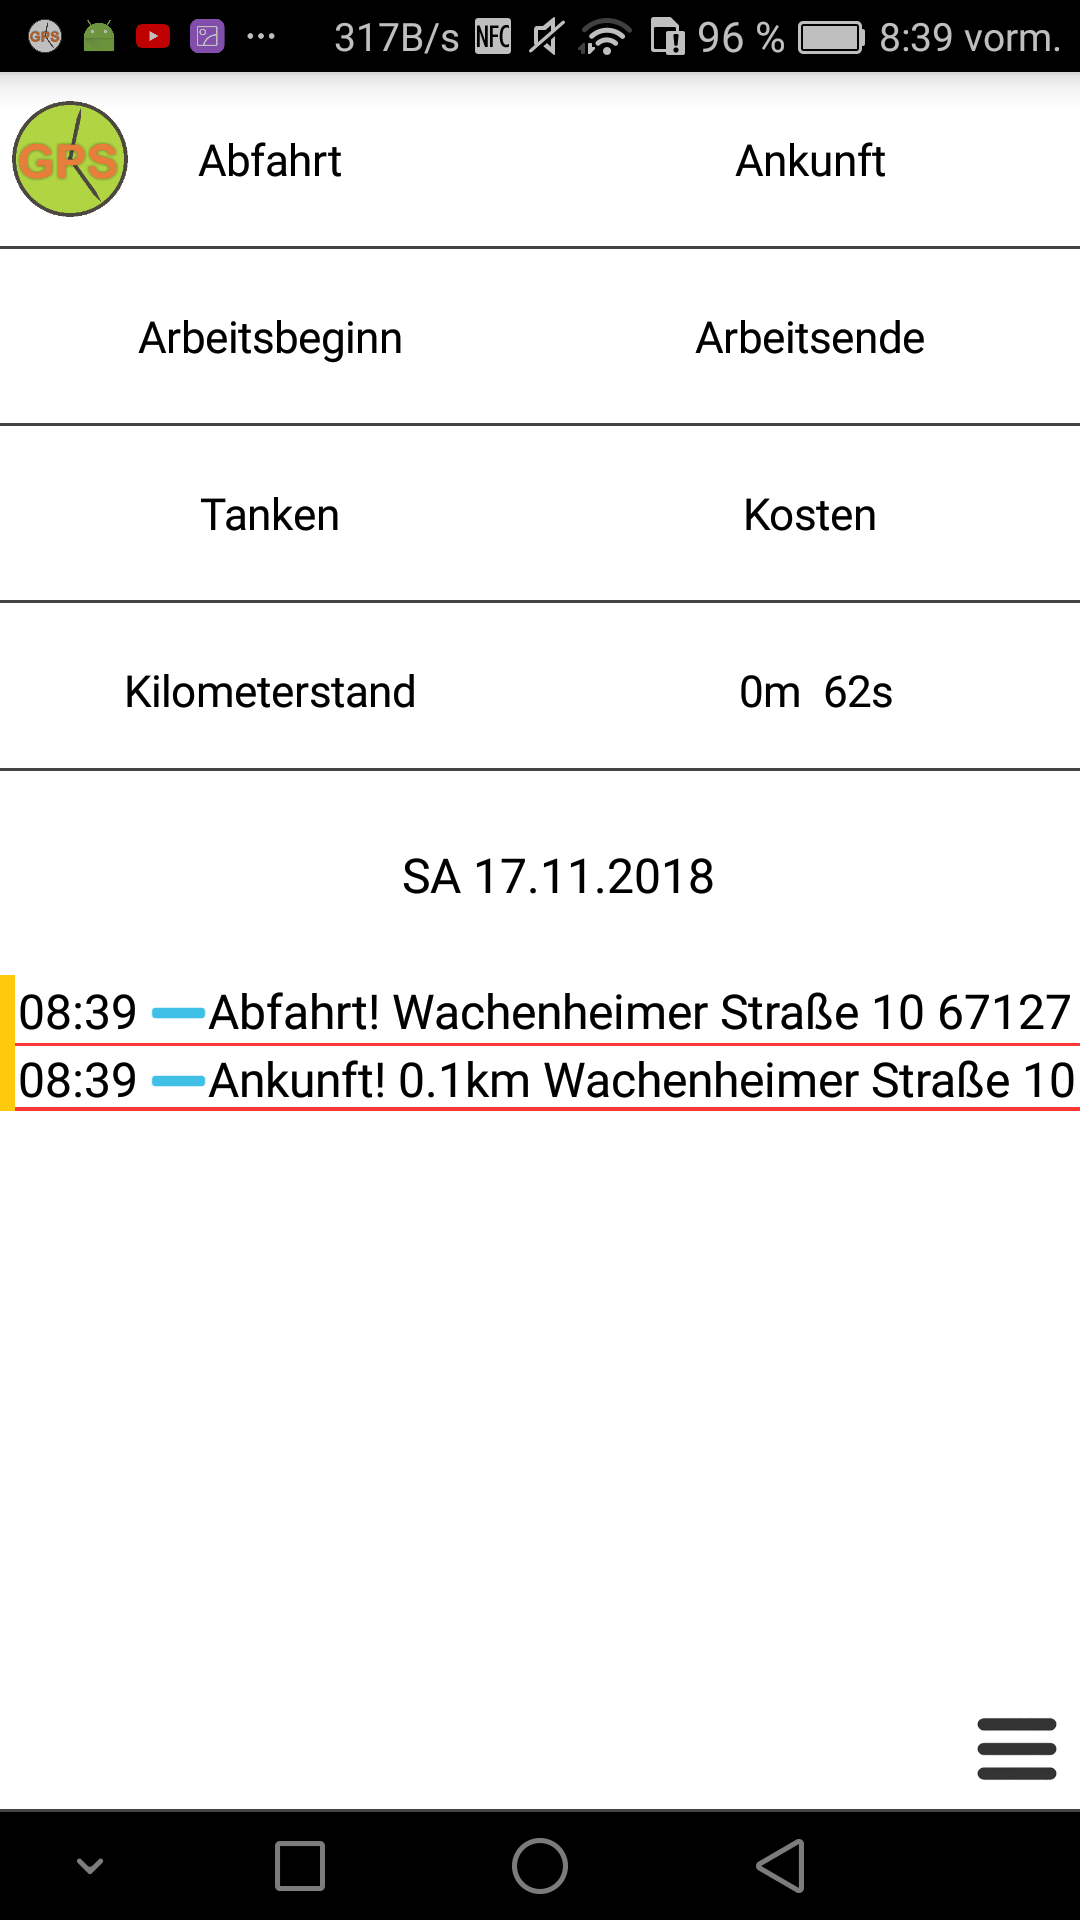
\includegraphics[scale=0.14]{img/gps1}
        \caption{\label{img:img/gps1}GPS Z+F Startbildschirm.}
    \end{minipage}
    \hspace{0.1\linewidth}% Abstand zwischen Bilder
    \begin{minipage}[b]{.4\linewidth} % [b] => Ausrichtung an \caption
        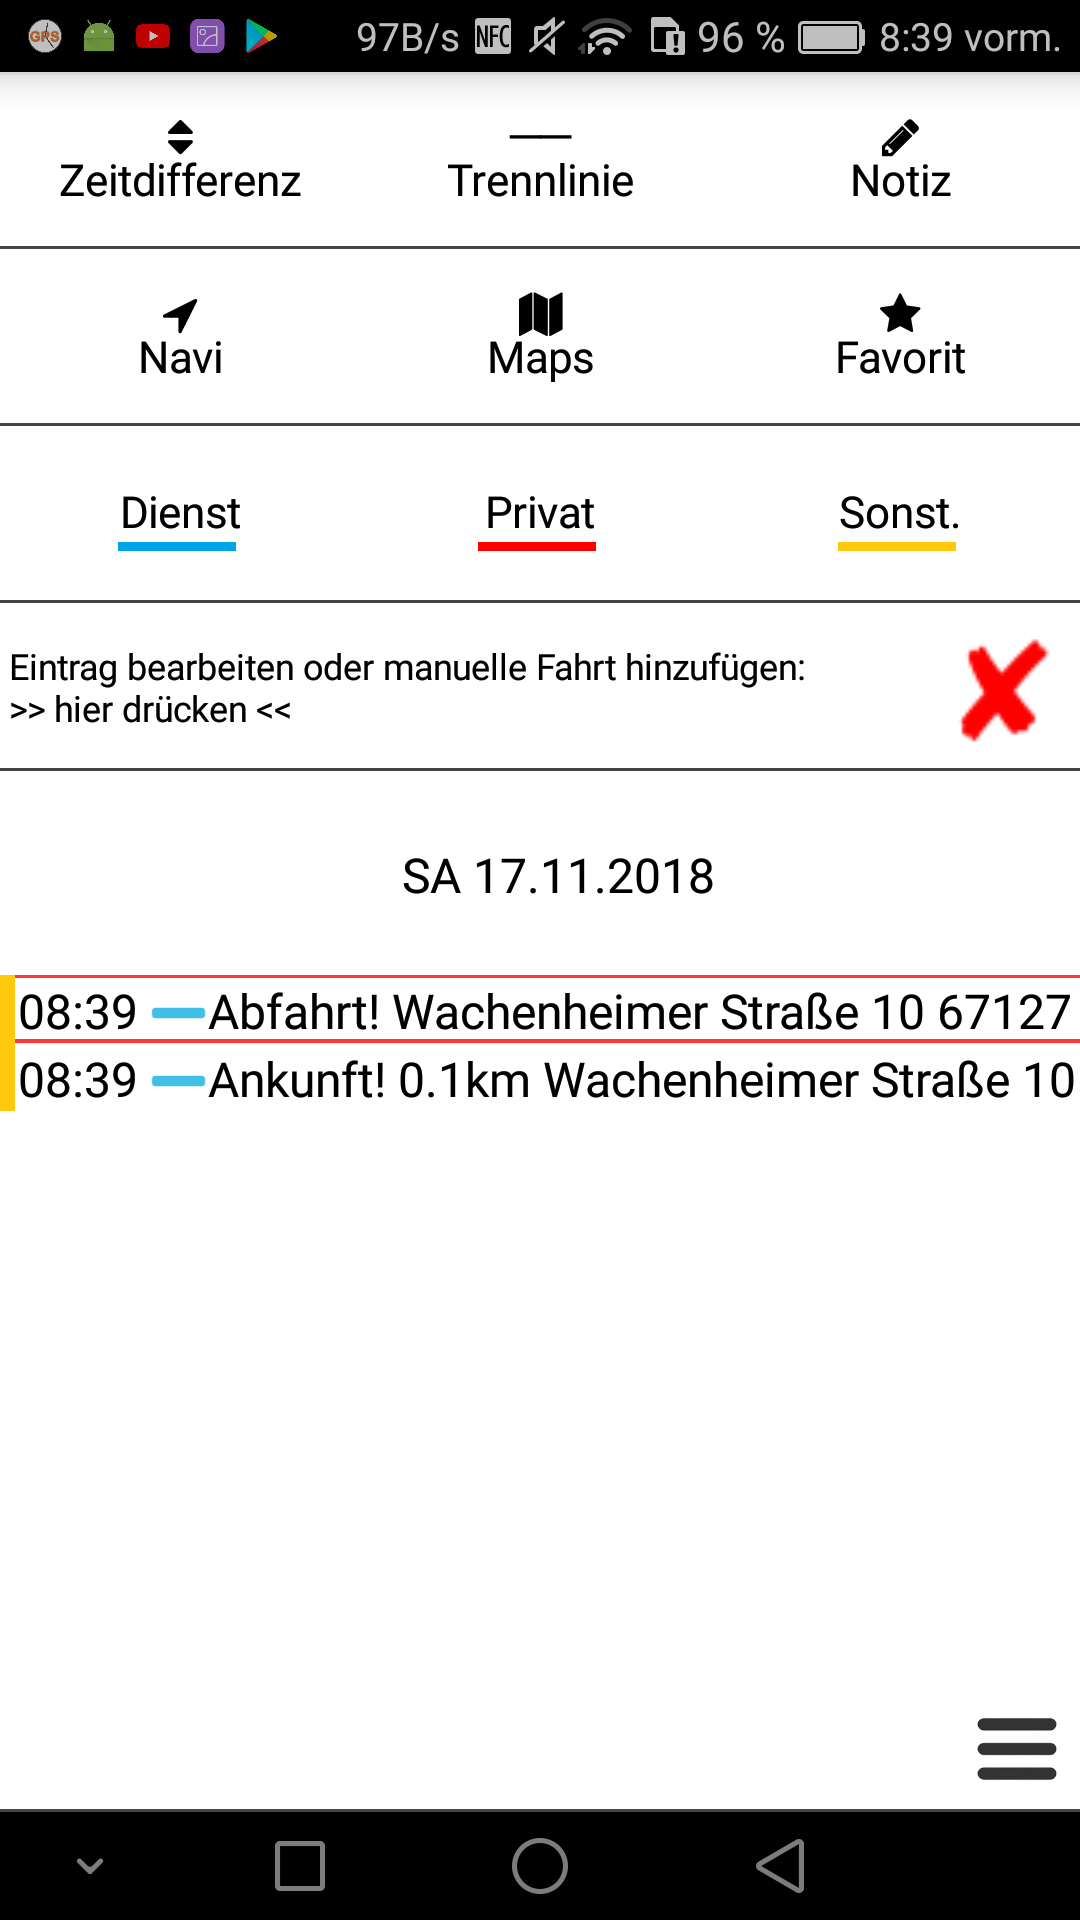
\includegraphics[scale=0.14]{img/gps2}
        \caption{\label{img:img/gps2}GPS Z+F Fahrt ausgewählt.}
    \end{minipage}
\end{figure}

\begin{figure}[H]%zwei bilder nebeneinander
    \begin{minipage}[b]{.4\linewidth} % [b] => Ausrichtung an \caption
        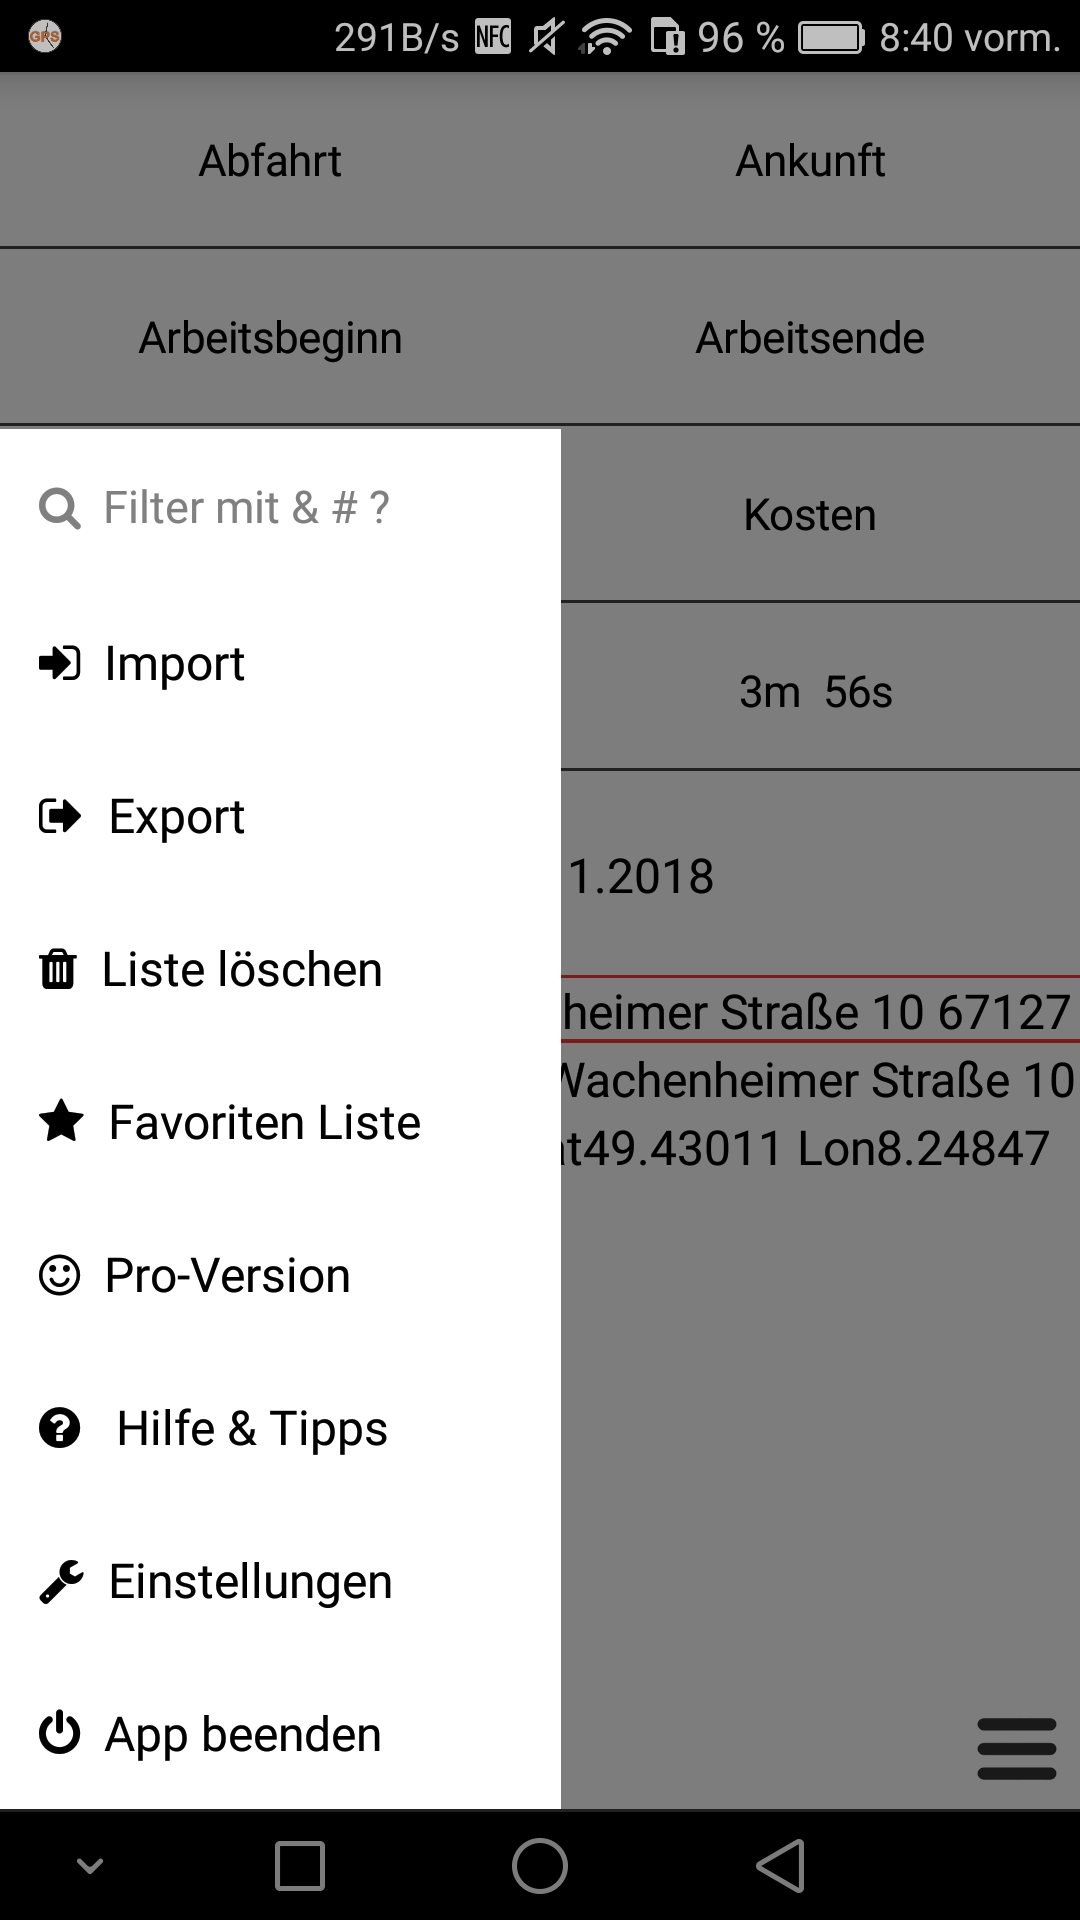
\includegraphics[scale=0.14]{img/gps3}
        \caption{\label{img:img/gps3}GPS Z+F Einstellungen.}
    \end{minipage}
    \hspace{0.1\linewidth}% Abstand zwischen Bilder
    \begin{minipage}[b]{.4\linewidth} % [b] => Ausrichtung an \caption
        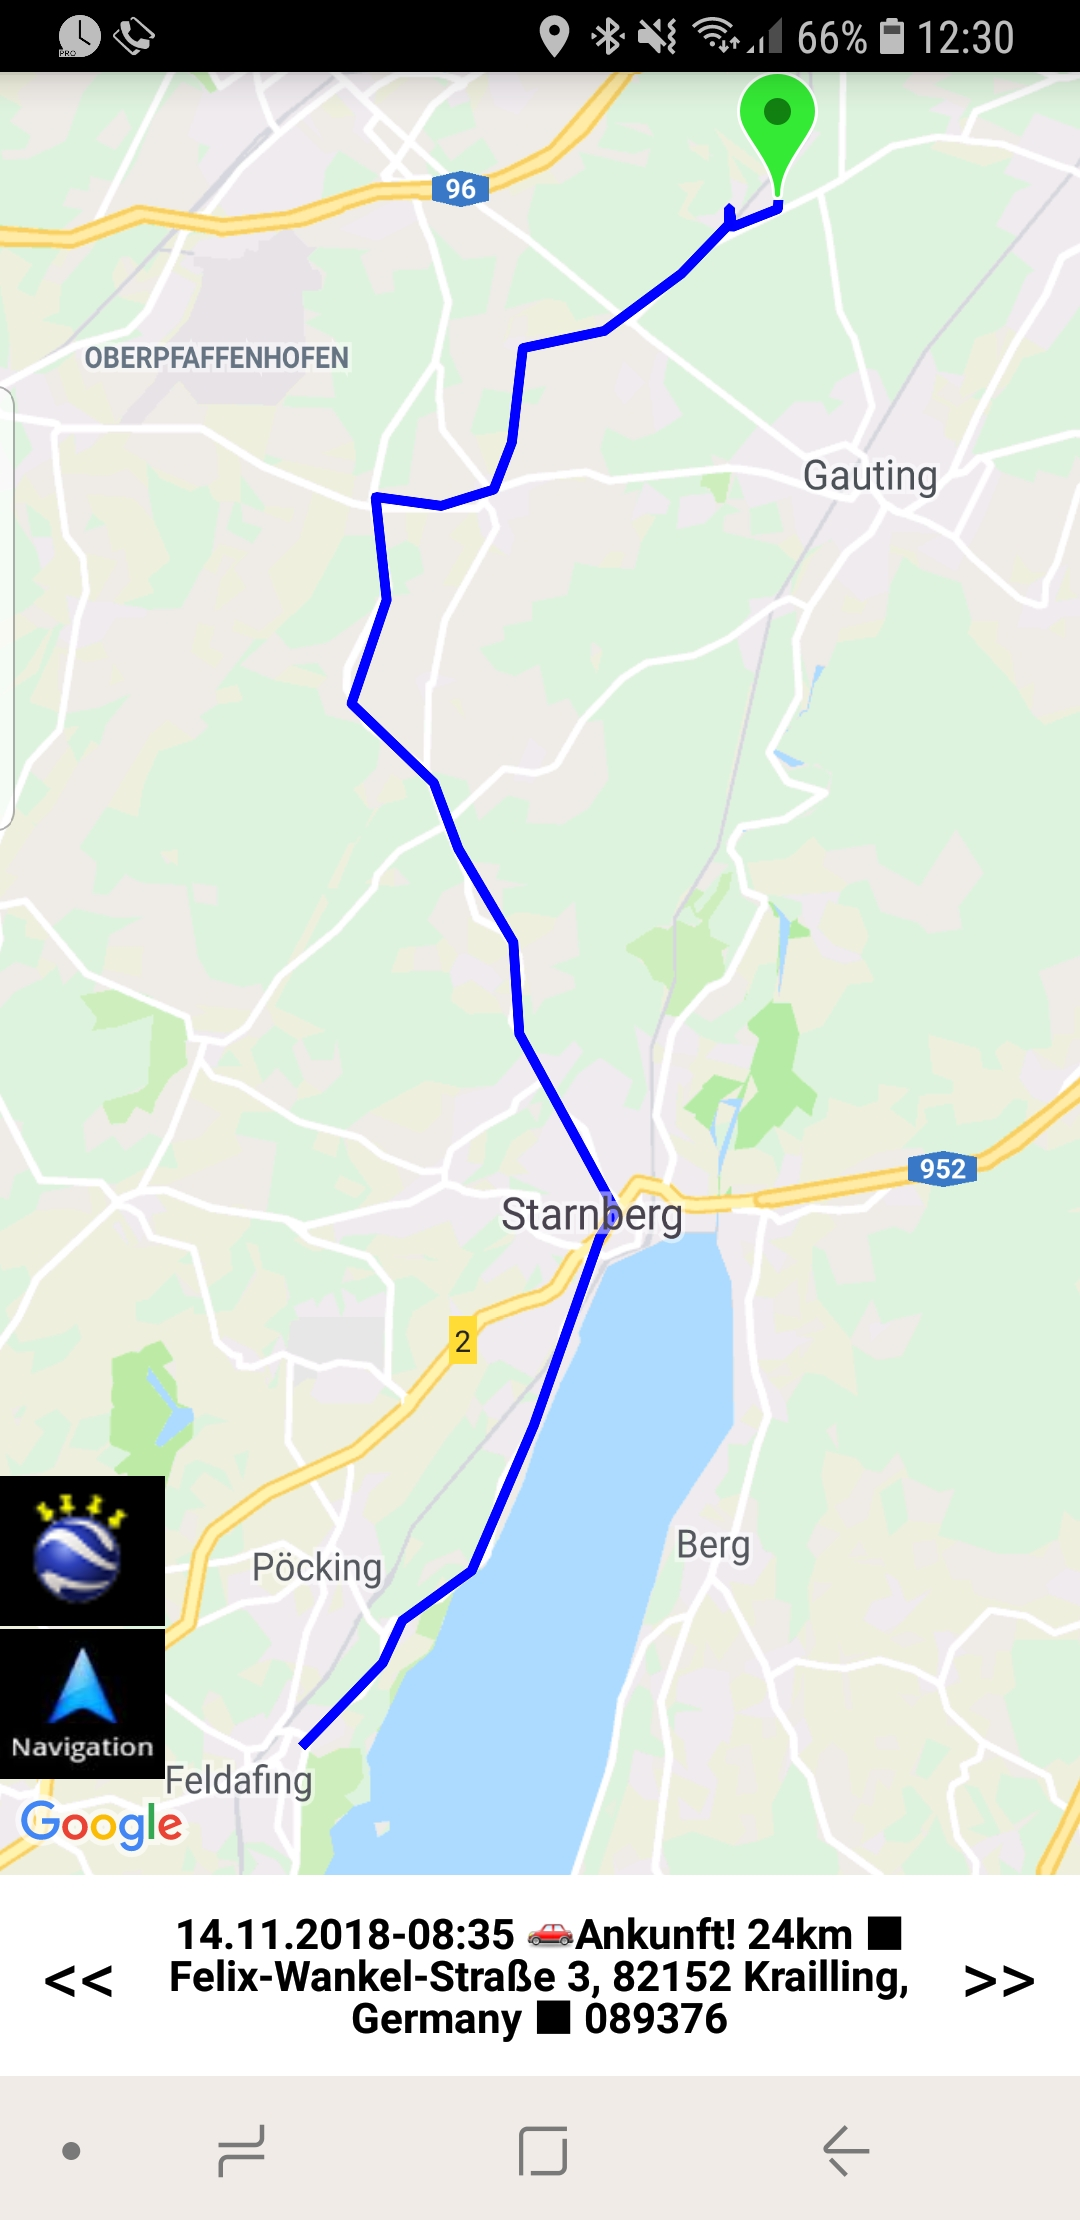
\includegraphics[scale=0.14]{img/gps4}
        \caption{\label{img:img/gps4}GPS Z+F aufgezeichnete Fahrt auf Karte.}
    \end{minipage}
\end{figure}

\subsubsection{Kommentare im Play Store}
\begin{enumerate}
    \item Der automatische Start und Ende der Aufzeichnungen ist sehr gut.
    \item Nicht Finanzamt konform da Änderungen nicht nachvollziehbar sind (nur in der Pro Version).
    \item Bedienung nicht induitiv.
\end{enumerate}

\subsubsection{Fazit}
Diese App ist im punkte Funktionalität woll die beste Lösung die es ohne Abo gibt. Aber designtechnisch
sehe ich noch Verbesserungspotential. Die Hälfte des Bildschirms besteht nur aus Buttons, die Liste
der erfassten Fahrten ist sehr klein und der optionen Button im rechten unteren Eck entspricht nicht
den Style-Guides. Außerdem wird der Eintrag sofort gelöscht wenn man auf löschen klickt. Gut ist die
Ansicht der Routen auf einer Karte.

\subsection{kfz fahrtenbuch}
Diese App wurde über 10.000 mal heruntergeladen und befindet sich damit im mittelfeld von den von mir
analysierten Apps. Durchschnittlich wurde die App mit 2,9 Sternen bei 52 Rezessionen bewertet.
Diese App wird in Verbindung mit einer Cloud Lösung mit einer Web Anwendung angeboten und ist mit einem
monatlichen Abo verbunden. Wenn man die kostenlose Version benutzt kann man nur Fahrten per Hand eintragen.

\subsubsection{Design und Funktionalität}
Auf \ref{img:img/kfz1} sehen Sie den Startbildschirm. Auf diesem gibt es drei Buttons, \textit{Fahrt aufzeichnen},
\textit{Fahrt erfassen} und \textit{Fahrten bearbeiten}. Die möglichkeit eine Fahr aufzuzeichnen gibt es nur
wenn man ein Abo abgeschlossen hat. \ref{img:img/kfz2} zeigt einen Scrennshot aus dem Play Store wie die Oberfläche
einer solchen Aufzeichnung aussieht. Da ich keine möglichkeite hatte die Funktion selbst zu testen werde ich hier nicht
näher drauf eingehen. Klickt man auf den Button \textit{Fahrt erfassen} sieht man die Oberfläche aus \ref{img:img/kfz3}.
Ganz Oben kann man die Art der Fahr auswählen. In den underen Zeilen kann man Start-, Zieladresse, Distanz und Kilometerstand
eingeben. Klickt man auf dem Startbildschirm auf \textit{Fahrten bearbeiten} kommt man zum Verlauf (siehe \ref{img:img/kfz4}).
Hier gibt es eine wie ein Zeitstrahl aufgebaute Ansicht aller fahrten. Bei Bedarf kann man erfasste Fahrten vervollständigen,
dazu öffnet sich wieder die selbe Oberfläche wie zum erfassen einer Fahrt.

\begin{figure}[H]%zwei bilder nebeneinander
    \begin{minipage}[b]{.4\linewidth} % [b] => Ausrichtung an \caption
        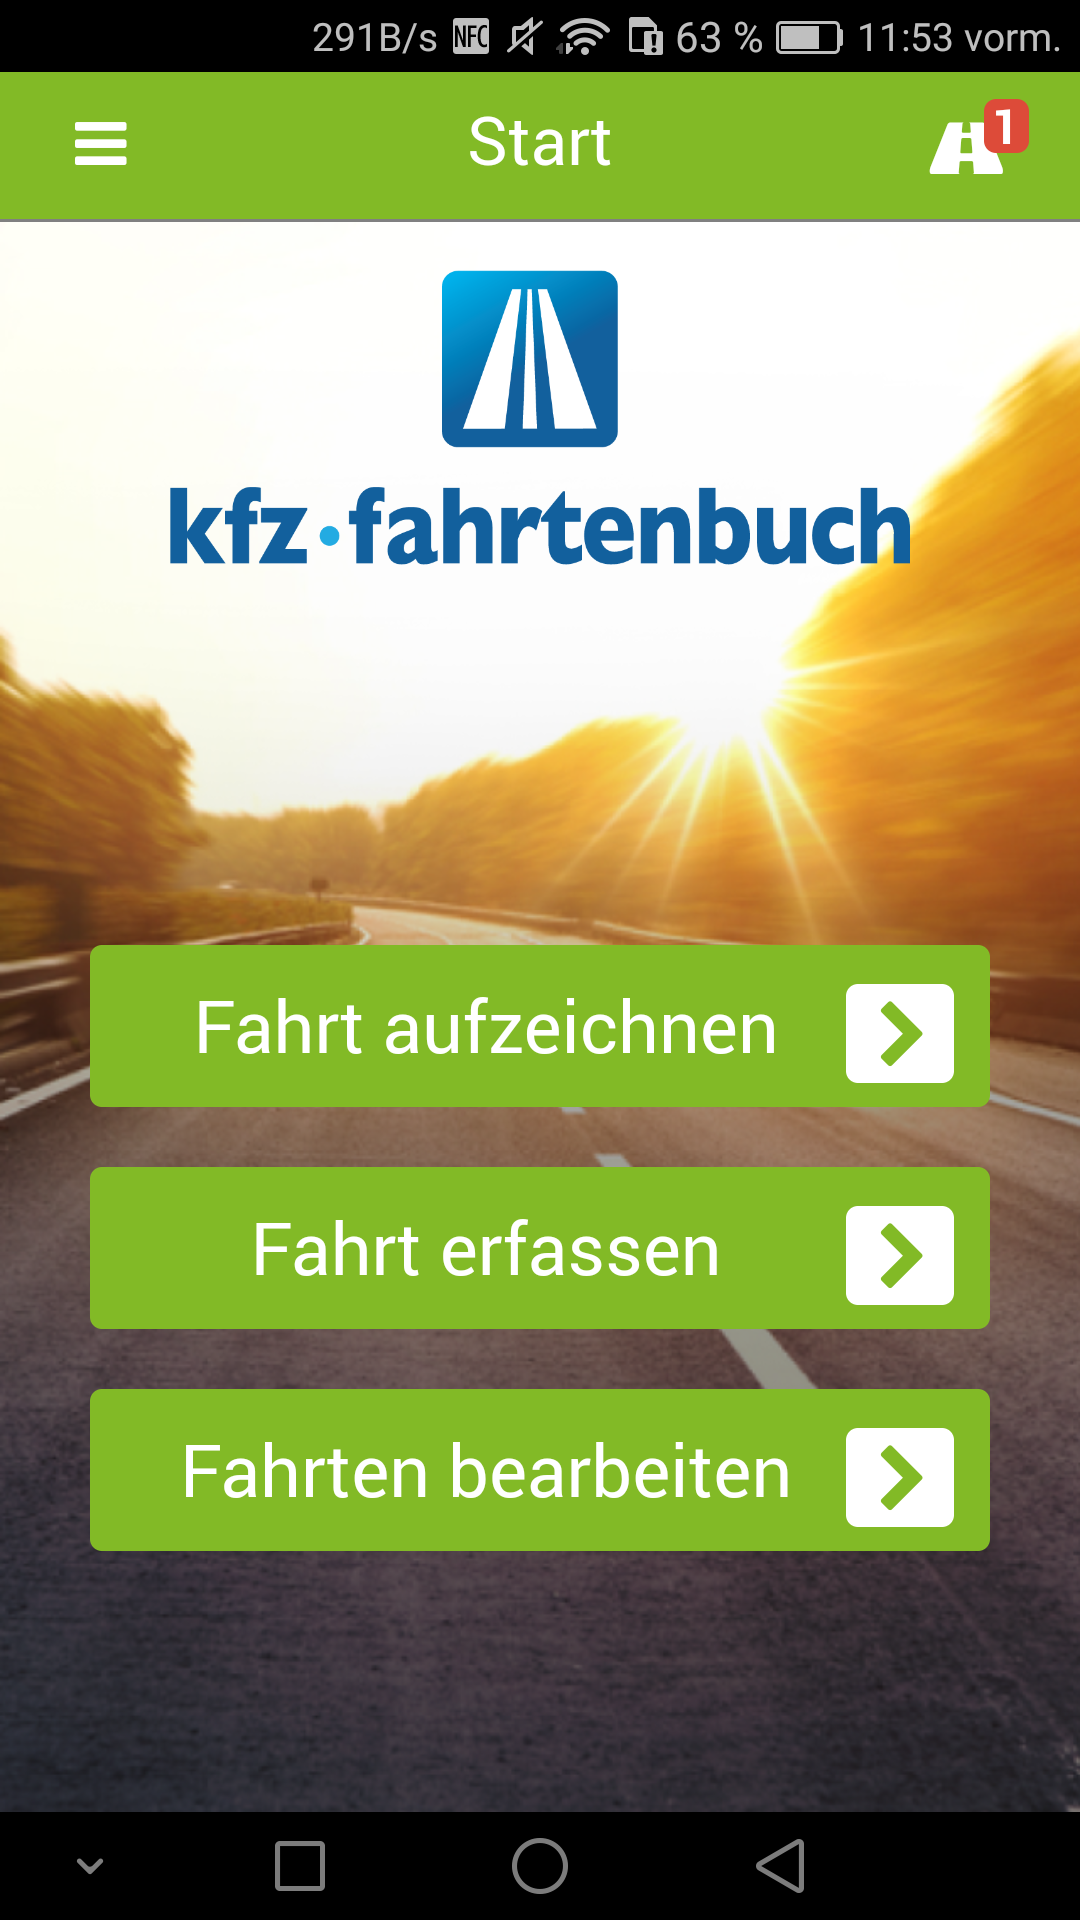
\includegraphics[scale=0.14]{img/kfz1}
        \caption{\label{img:img/kfz1}kfz Fahrtenbuch: Startbildschirm}
    \end{minipage}
    \hspace{0.1\linewidth}% Abstand zwischen Bilder
    \begin{minipage}[b]{.4\linewidth} % [b] => Ausrichtung an \caption
        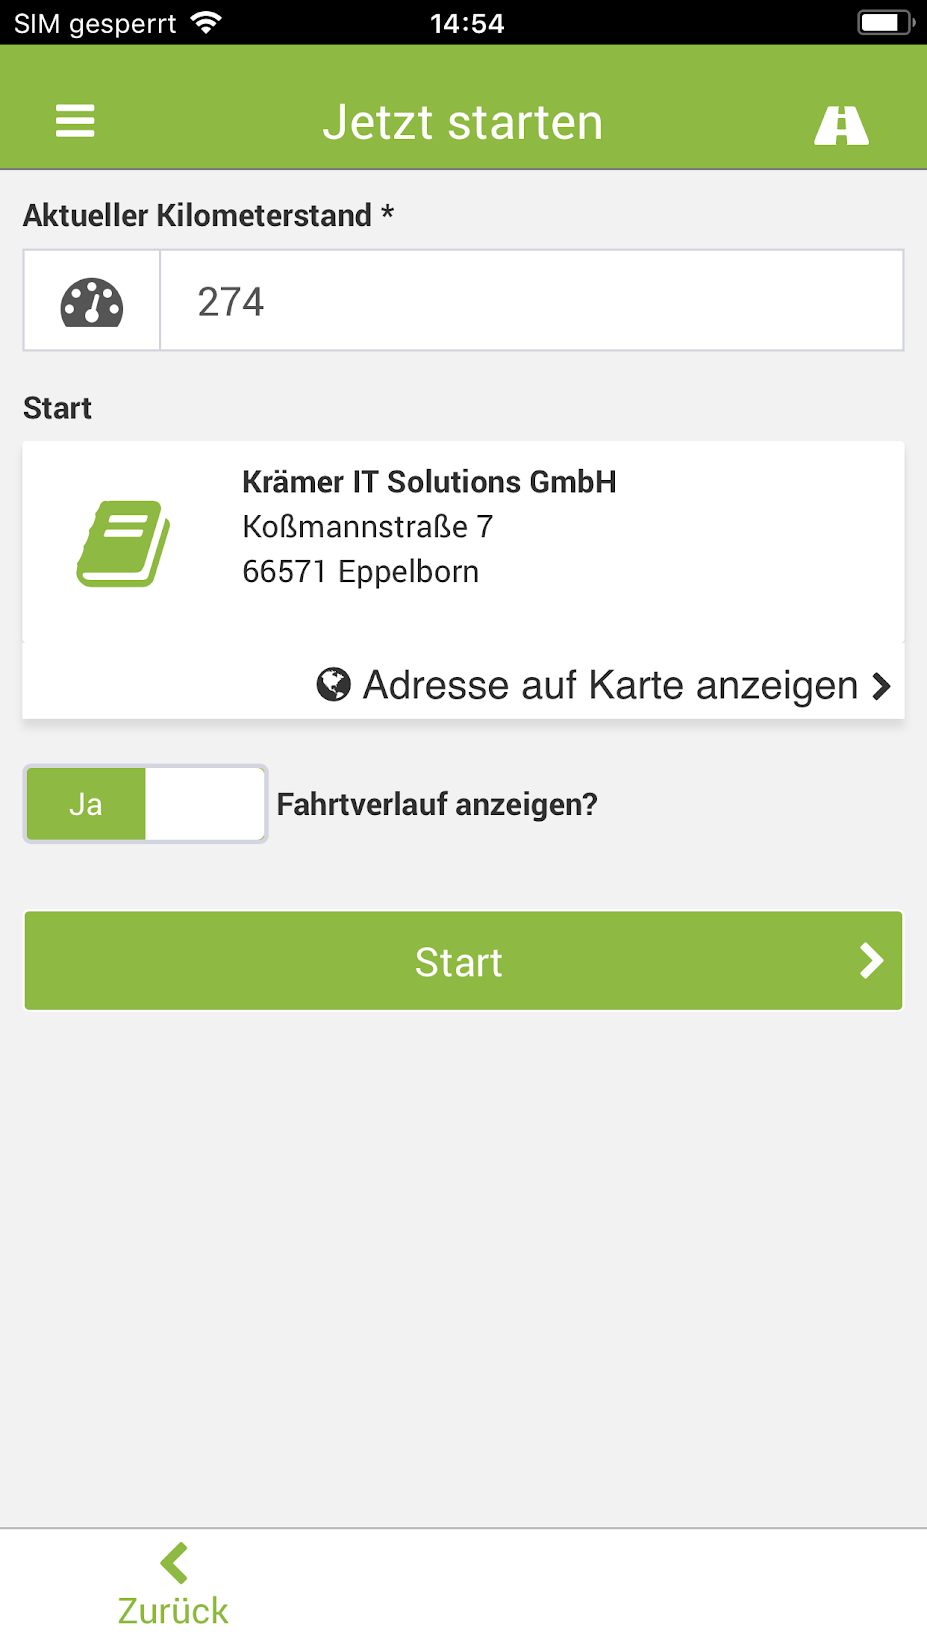
\includegraphics[scale=0.17]{img/kfz2}
        \caption{\label{img:img/kfz2}kfz Fahrtenbuch: fahrt aufzeichnen}
    \end{minipage}
\end{figure}

\begin{figure}[H]%zwei bilder nebeneinander
    \begin{minipage}[b]{.4\linewidth} % [b] => Ausrichtung an \caption
        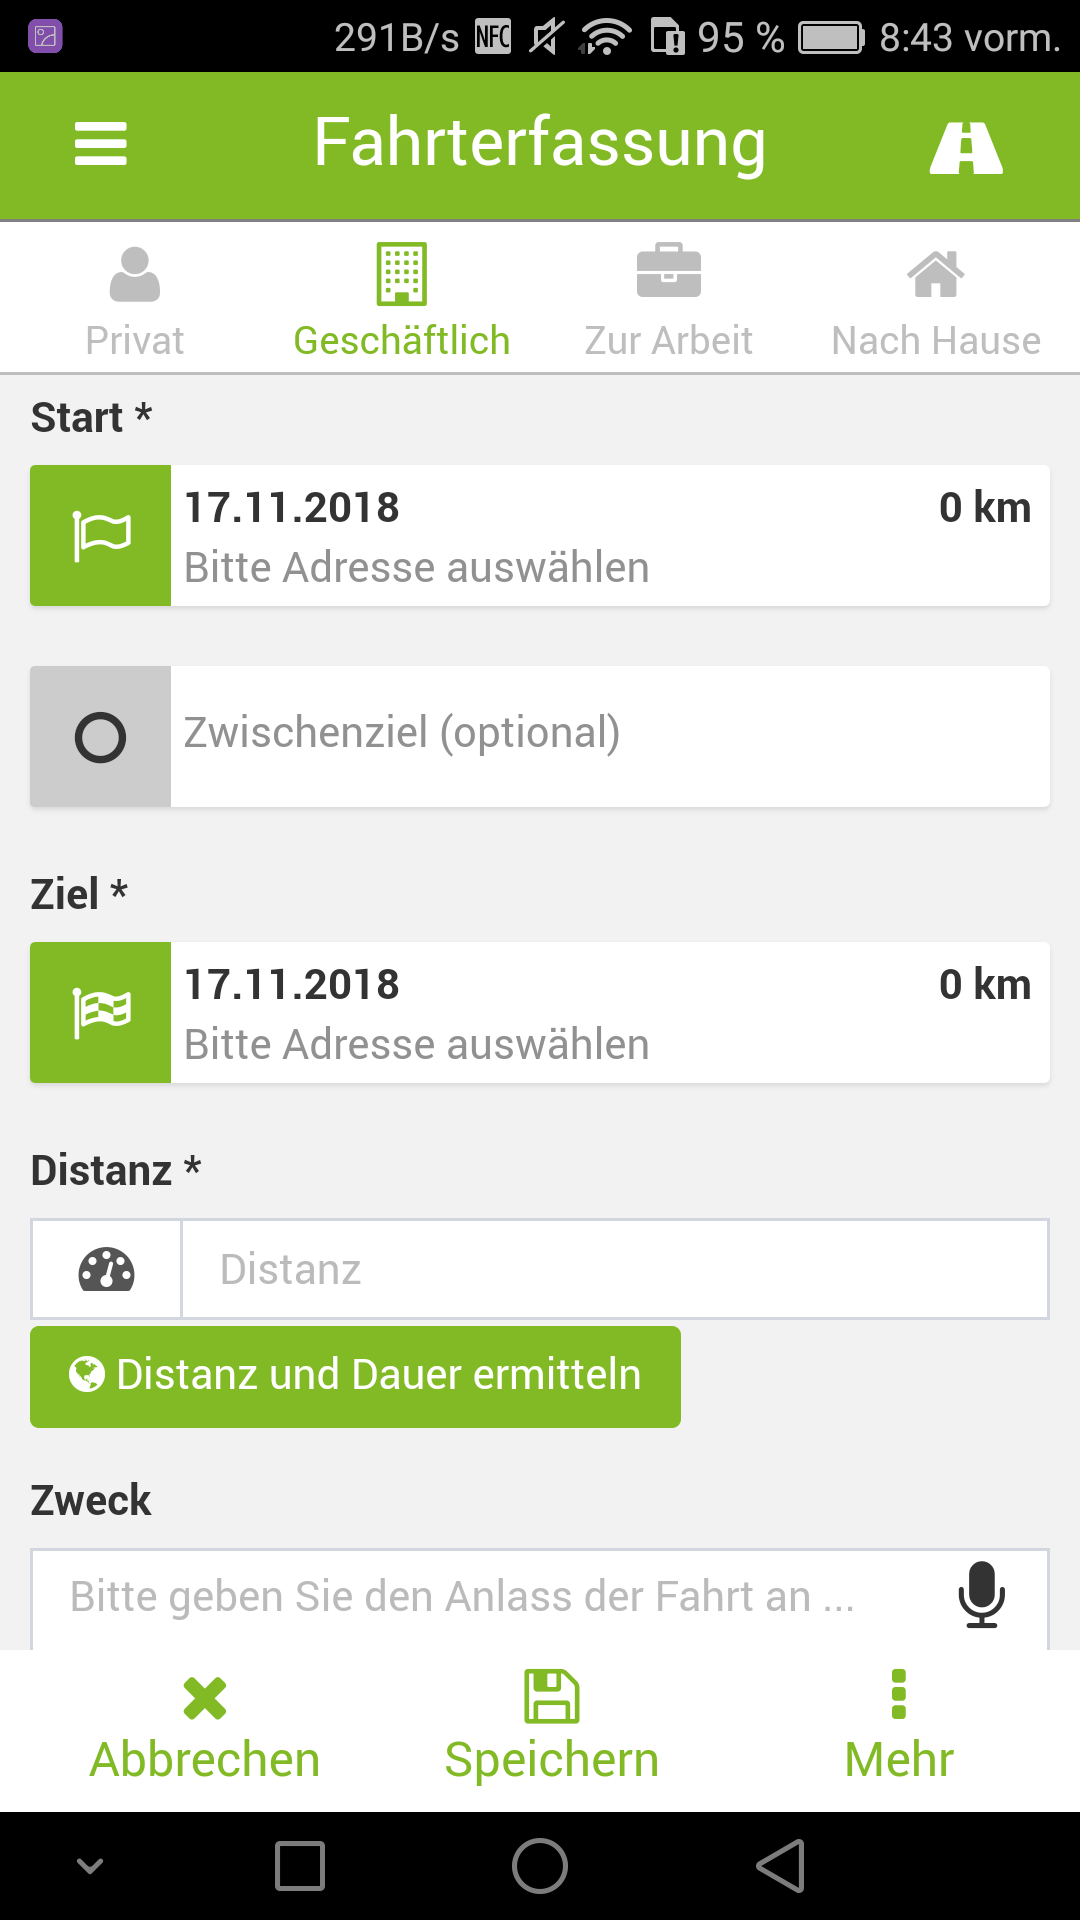
\includegraphics[scale=0.14]{img/kfz3}
        \caption{\label{img:img/kfz3}kfz Fahrtenbuch: fahrt erfassen}
    \end{minipage}
    \hspace{0.1\linewidth}% Abstand zwischen Bilder
    \begin{minipage}[b]{.4\linewidth} % [b] => Ausrichtung an \caption
        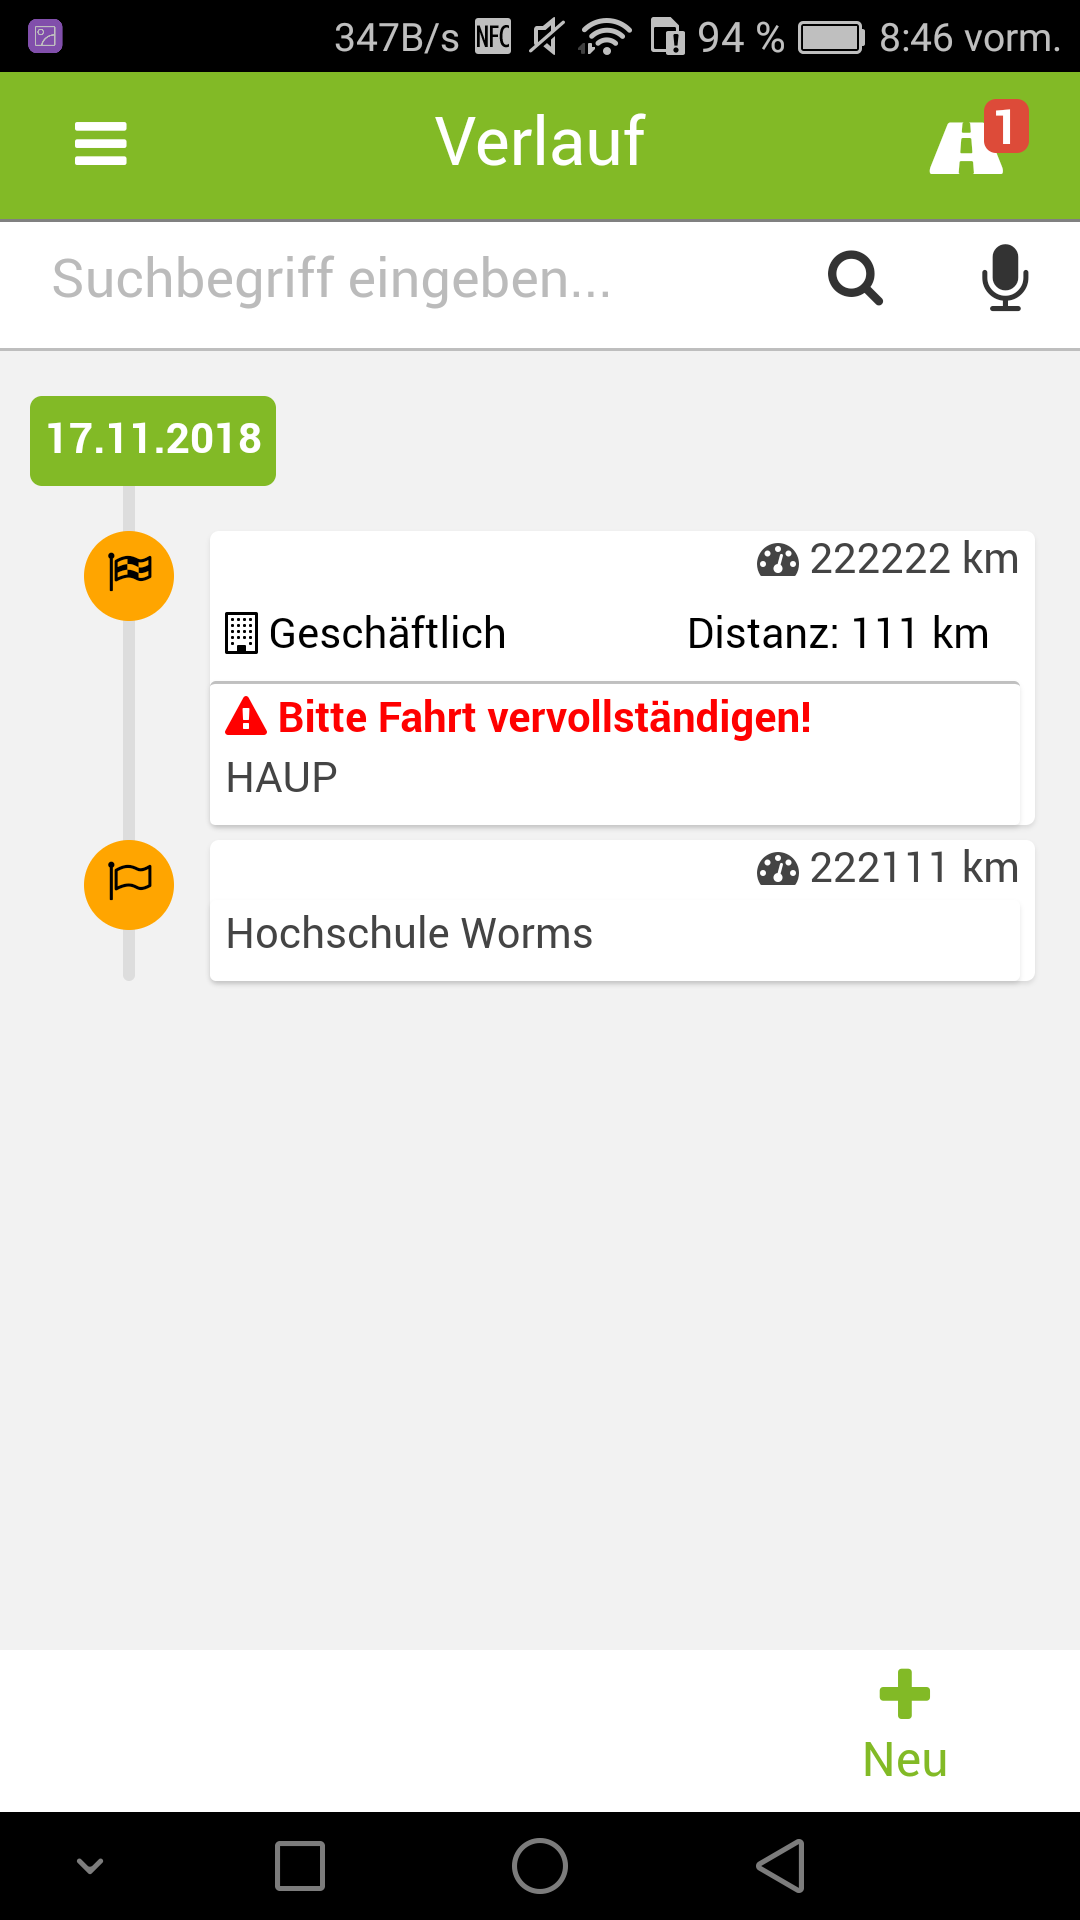
\includegraphics[scale=0.14]{img/kfz4}
        \caption{\label{img:img/kfz4}kfz Fahrtenbuch: fahrt bearbeiten}
    \end{minipage}
\end{figure}

\subsubsection{Kommentare im Play Store}
Pries Leistung Verhältnis der Cloud LÖsung wird kritisiert
\begin{enumerate}
    \item
\end{enumerate}

\subsubsection{Fazit}
Die Funktionalität in der kostenlosen Version ist sehr eingeschränkt und bietet nicht einmal die
Möglichkeit der Aufzeichnung durch GPS. Das Design der Oberfläche ist moderner und übersichtlicher
im Vergleich zu der ersten App. ABer wenn man die eingeschränkte Funktionalität in der kostenlosen
Version berücksichtigt halte ich diese App im Vergleich für die schlechteste, was auch die Bewertungen
im Play Store wiederspiegeln.

\subsection{SquareTrip}
Square Trip hat durchschnittlich 4,1 Sterne bei 118 Rezessionen bekommen und wurde über 10.000
mal heruntergeladen. Es gibt eine kostenlose und eine Pro Version.


\subsubsection{Design und Funktionalität}
\ref{img:img/squ1} zeigt den Startbildschirm der App beim ersten Starten und \ref{img:img/squ2} die Ansicht wenn 
schon Fahrten erfasst wurden. Im ersten oberen drittel sieht gibt es ganz links einen Button um zwischen den Ansichten zu wechseln.
Wenn man auf den \textit{Stern} klickt kann man erfasste fahrten zuordnen, wie in \ref{img:img/squ3}, ob es eine Private, 
Geschäftlichefahrt ode Arbeitsweg war.
In der Mitte gibt es ein Icon mit dem man seine Autos verwalten kann. Zum Verwalten der Autos kann man ein Bild hinzufügen, 
Name/Modell angeben, Nummerschild und den Kilometerstand. Daneben kann man Fahrten anhand eines Filters suchen. Mit dem 
\textit{+} Symbol kann man eine neue Fahrt anlegen, siehe \ref{img:img/squ4}.
Die App erfasst fahrtren automatisch, das bedeutet sie läuft permanent im Hintergrund und wartet auf ein GPS-Signal.
Außerdem bittet die App die möglichkeit die letzte Parkposition seines Auto anzuzeigen und die
laufenden Kosten des Autos zu erfassen, da das für meine App aber eher uninteressant ist habe ich mir diese 
Funktionalitäten nicht näher angeschaut.  

\begin{figure}[H]%zwei bilder nebeneinander
    \begin{minipage}[b]{.4\linewidth} % [b] => Ausrichtung an \caption
        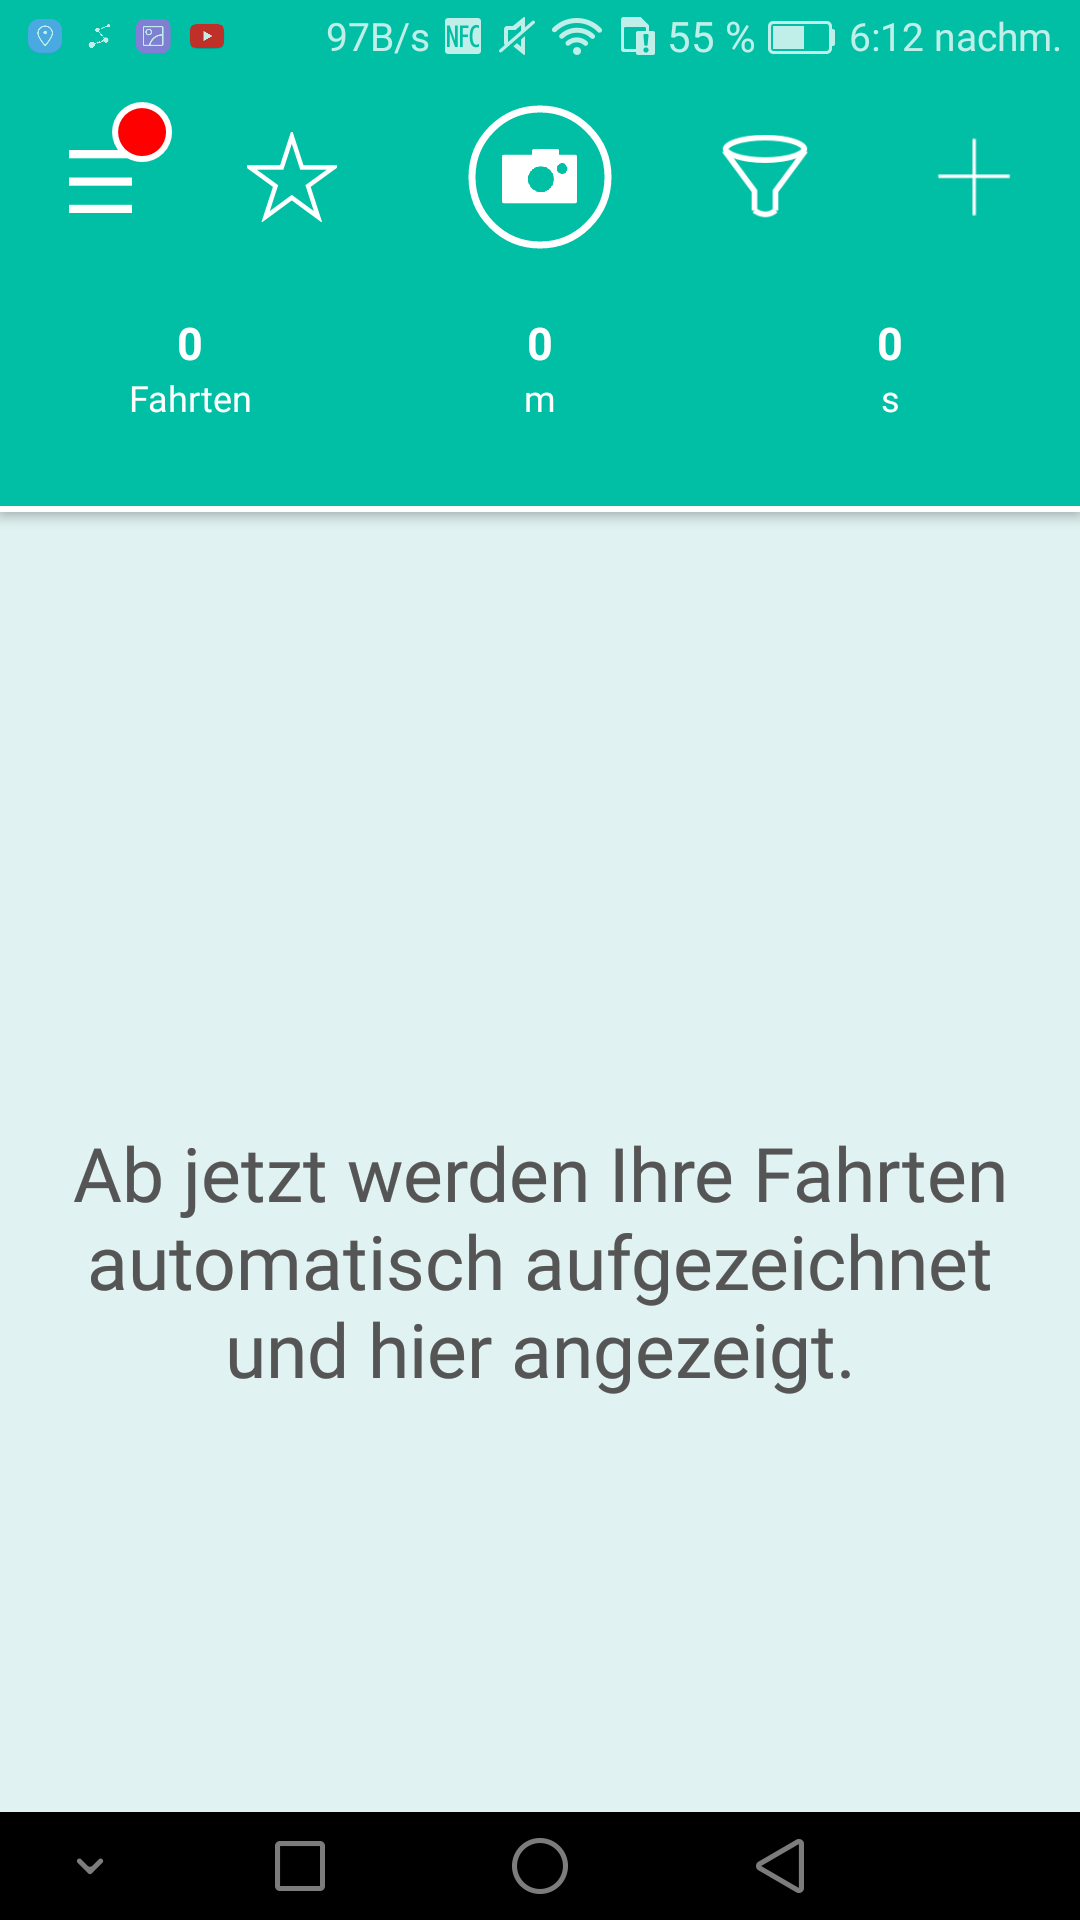
\includegraphics[scale=0.14]{img/squ1}
        \caption{\label{img:img/squ1}GPS Z+F Startbildschirm.}
    \end{minipage}
    \hspace{0.1\linewidth}% Abstand zwischen Bilder
    \begin{minipage}[b]{.4\linewidth} % [b] => Ausrichtung an \caption
        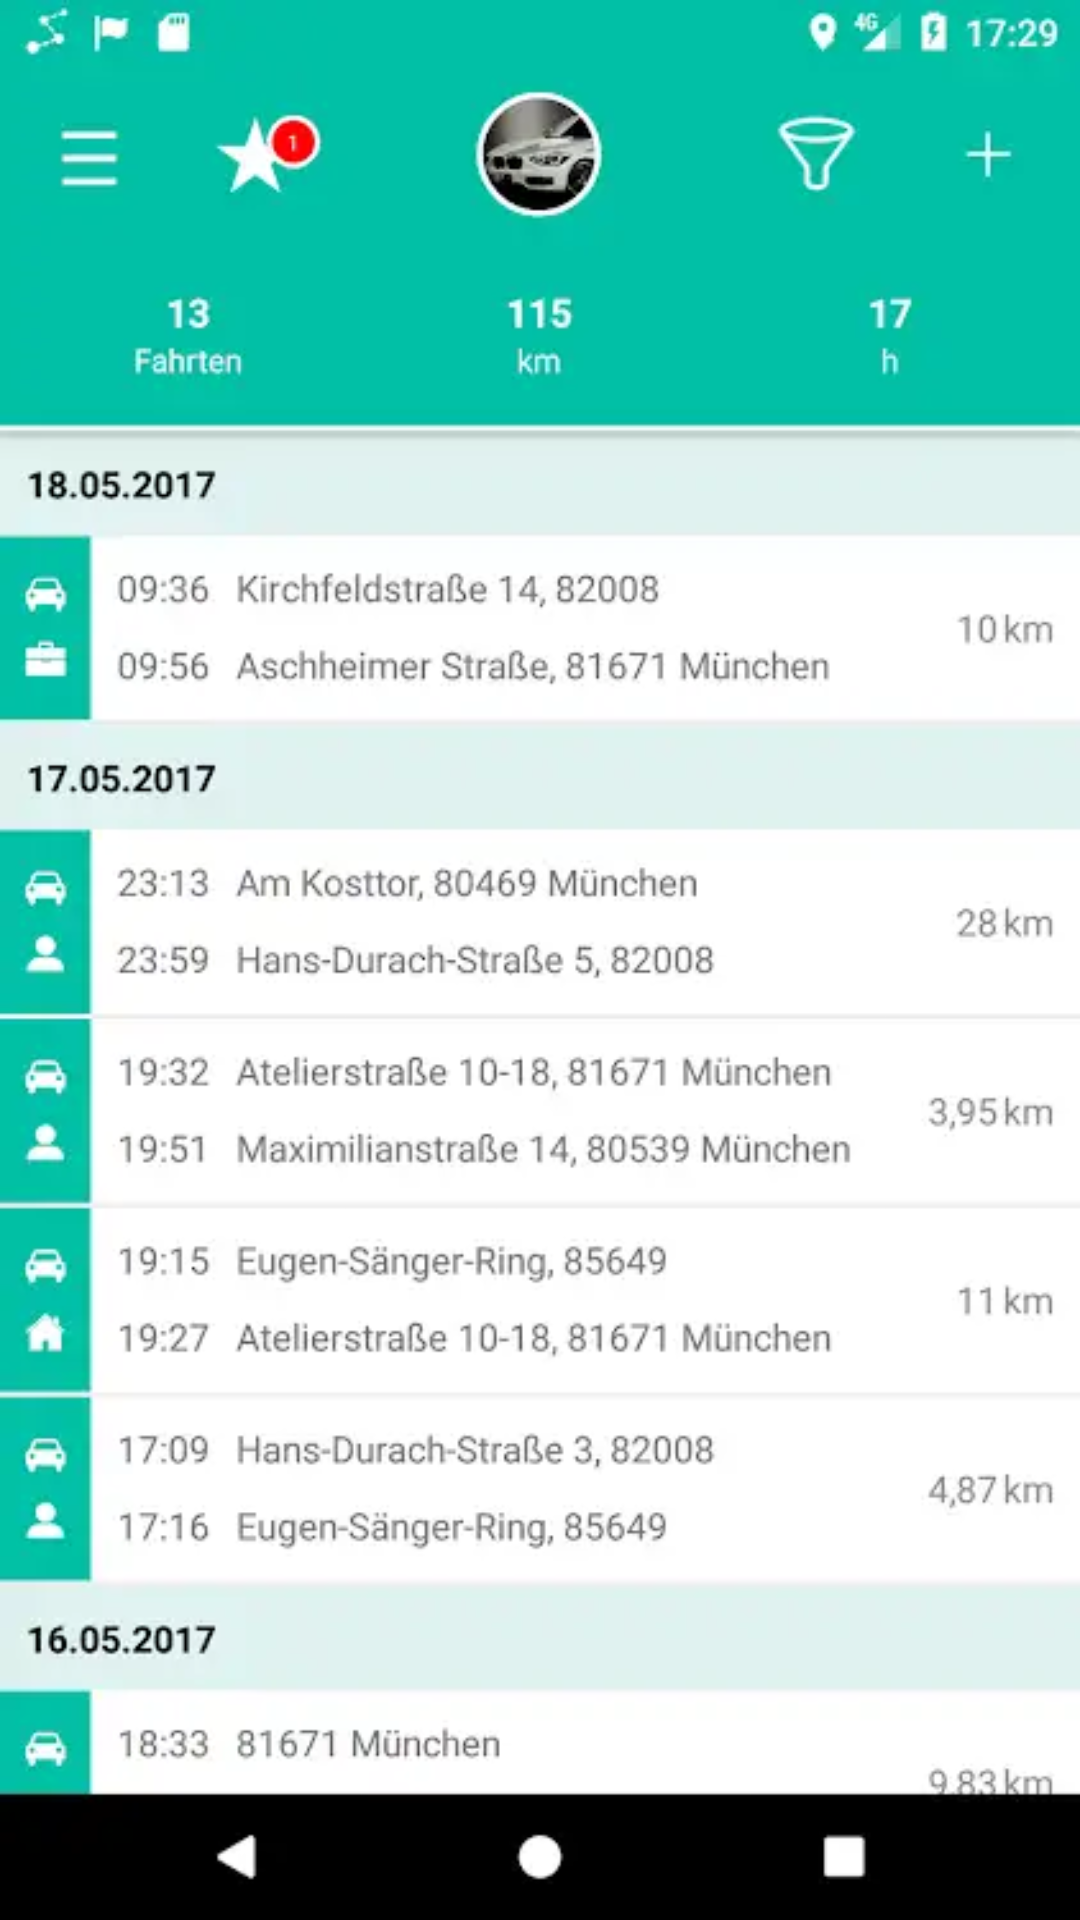
\includegraphics[scale=0.14]{img/squ2}
        \caption{\label{img:img/squ2}GPS Z+F Fahrt ausgewählt.}
    \end{minipage}
\end{figure}

\begin{figure}[H]%zwei bilder nebeneinander
    \begin{minipage}[b]{.4\linewidth} % [b] => Ausrichtung an \caption
        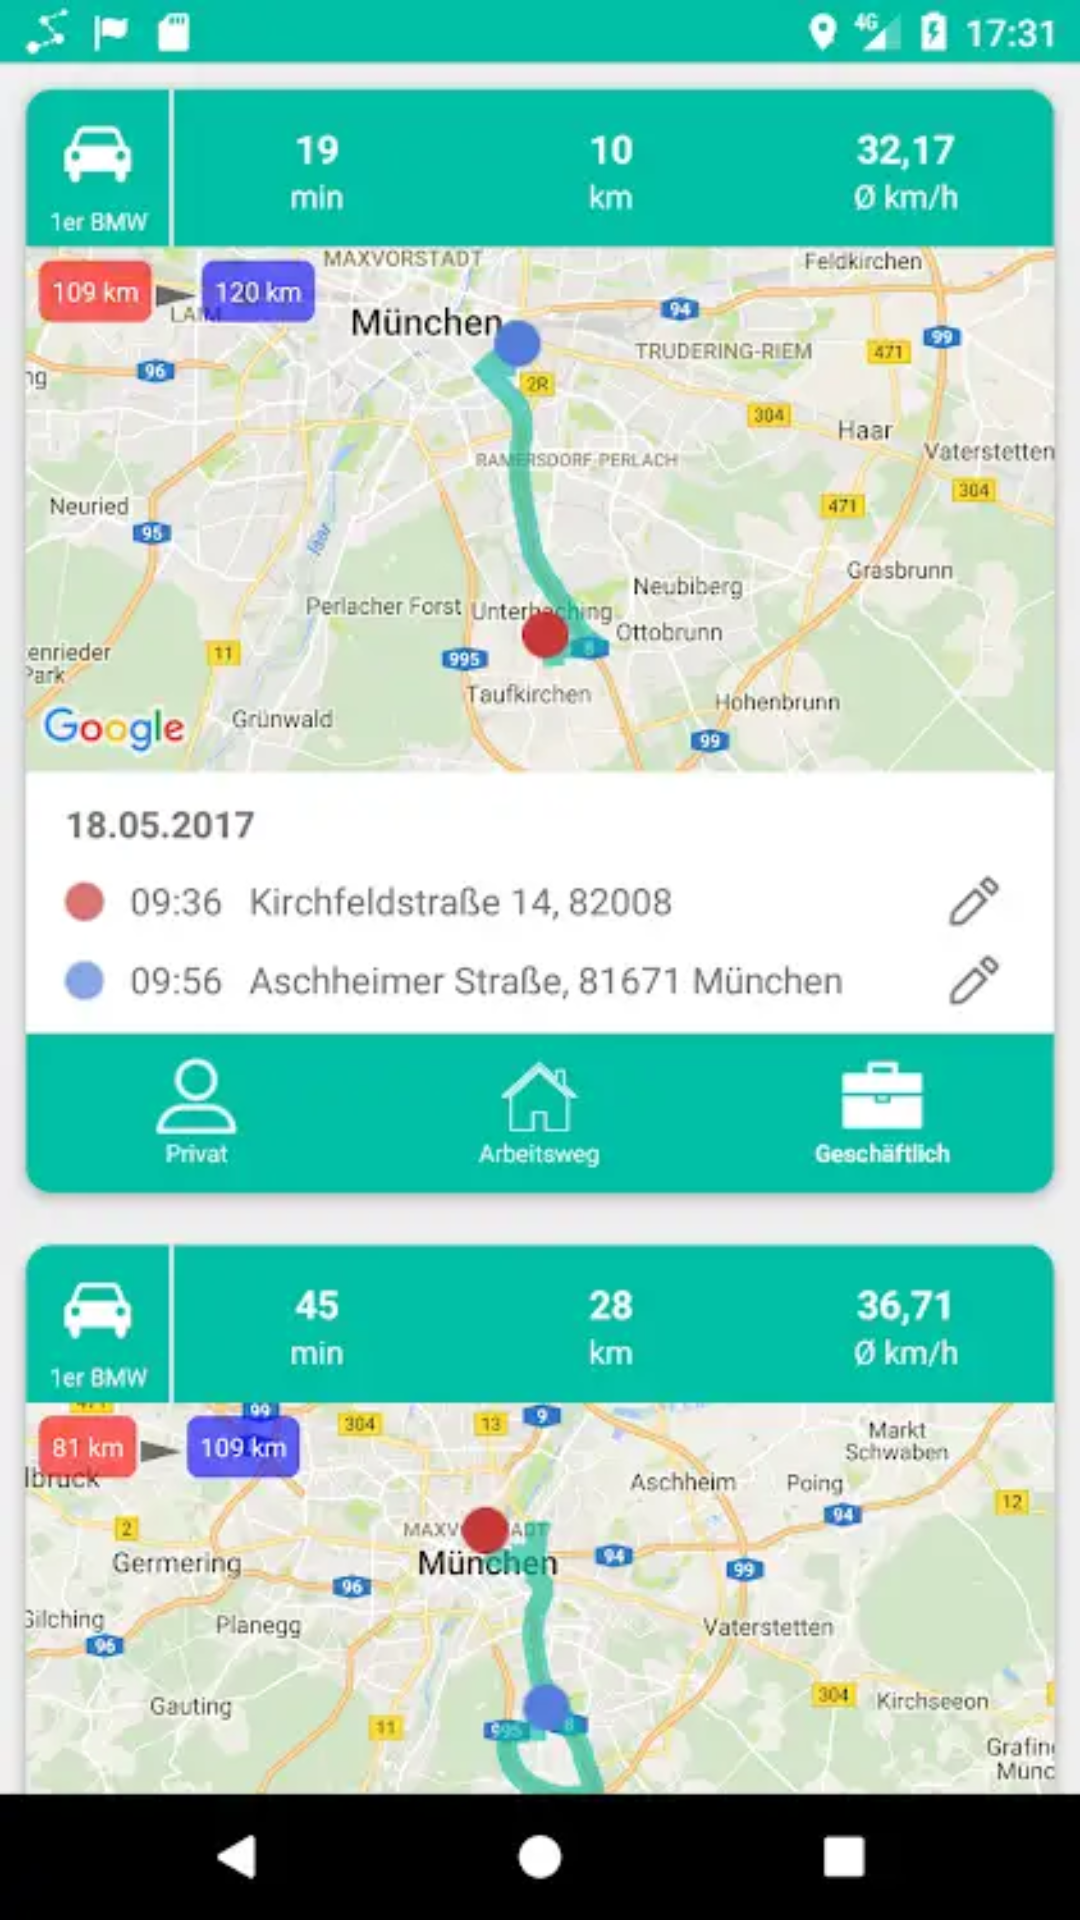
\includegraphics[scale=0.14]{img/squ3}
        \caption{\label{img:img/squ3}GPS Z+F Einstellungen.}
    \end{minipage}
    \hspace{0.1\linewidth}% Abstand zwischen Bilder
    \begin{minipage}[b]{.4\linewidth} % [b] => Ausrichtung an \caption
        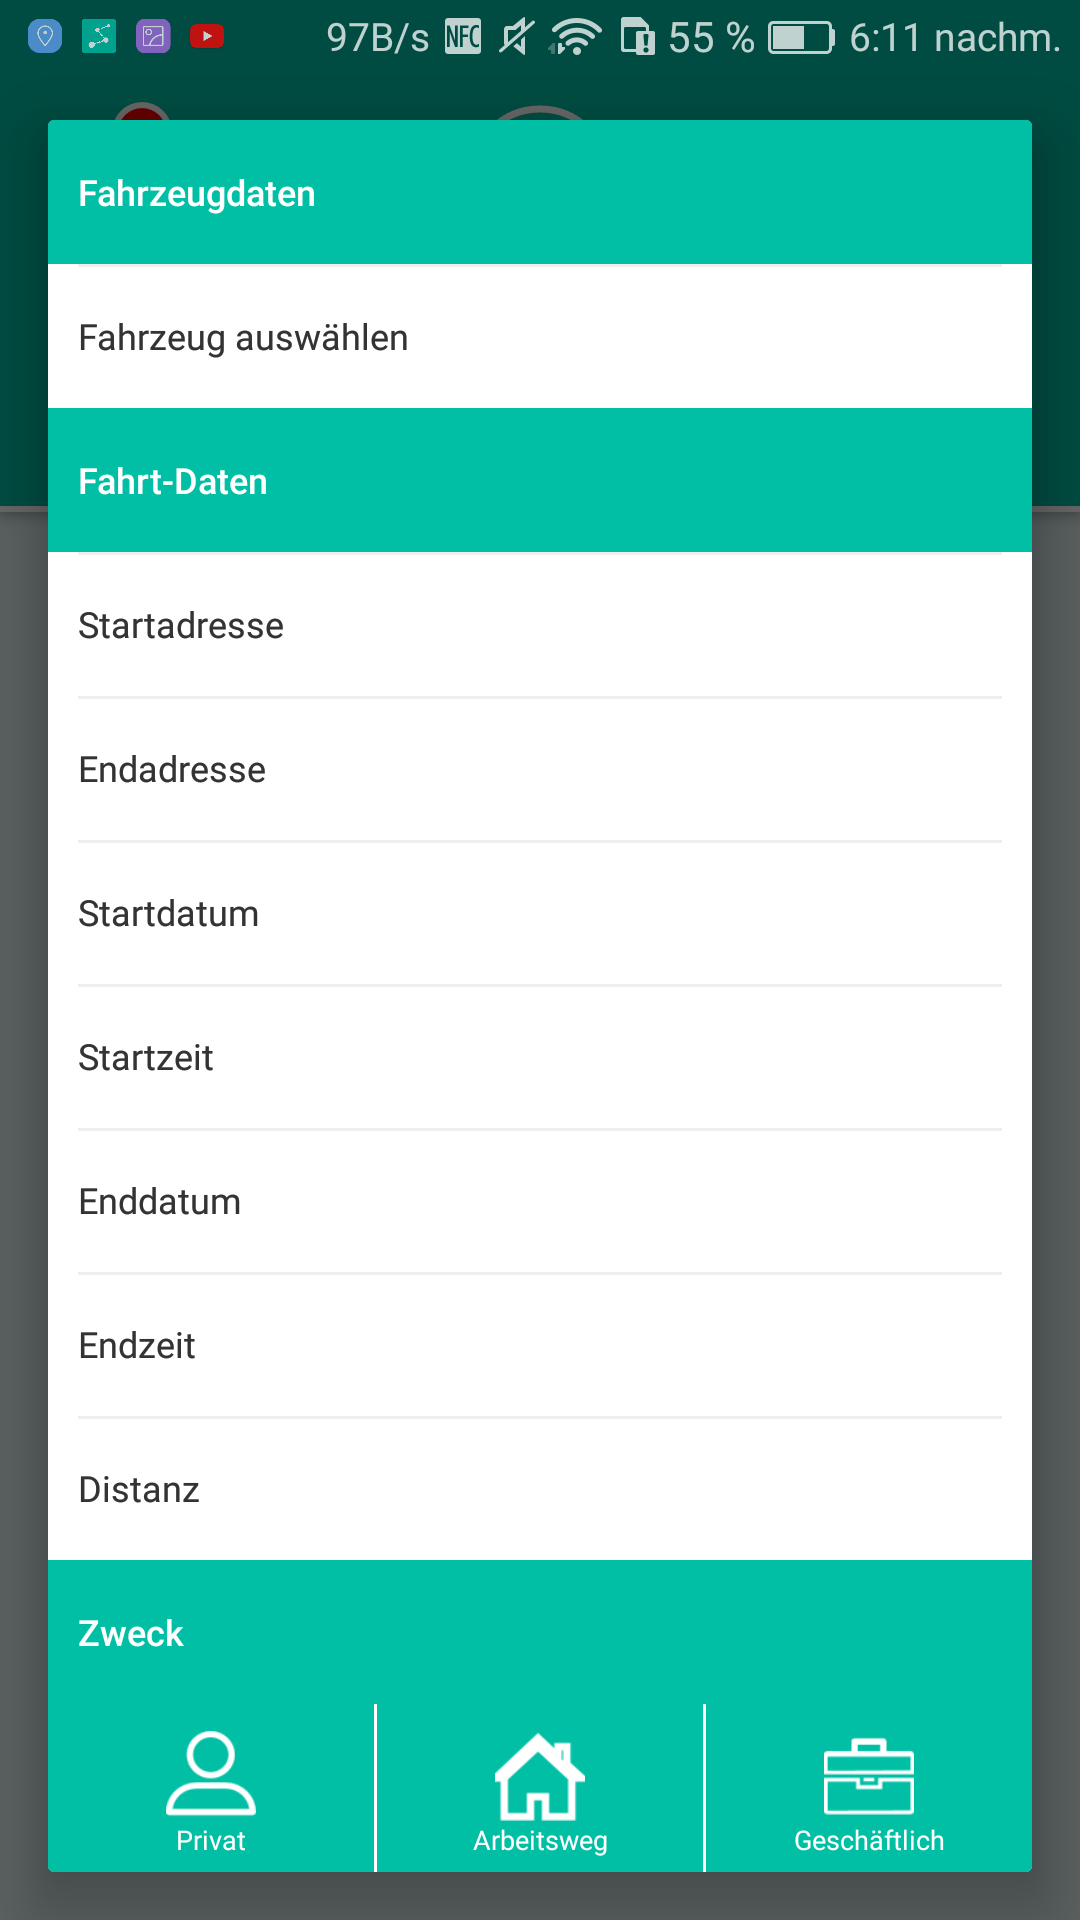
\includegraphics[scale=0.14]{img/squ4}
        \caption{\label{img:img/squ4}GPS Z+F aufgezeichnete Fahrt auf Karte.}
    \end{minipage}
\end{figure}

\subsubsection{Kommentare im Play Store}
\begin{enumerate}
    \item Die meisten Bewertungen sind zufrieden mit der App
\end{enumerate}

\subsubsection{Fazit}
Die Icons sind nicht unbedingt selbst erklärend. Das Design gefäält mir gut, die 
Deign Guidlines wurden eingehalten. Die App bietet auch die möglichkeit mehrere Autos zu verwalten, was 
aber für meine Zielgruppe eher uninteressant ist. Problematisch ist das die App permanent im Hintergrund läuft
und auf ein GPS-Signal wartet, was sich negativ auf die Akkuleistung auswirkt und außerdem gibt es keinen
Button zum starten einer Fahrt. Gut ist auch das die gefahrene Strecke auf einer Karte angezeigt wird.
Exportfunktionen gibt es nur in der Pro Version. 

\subsection{Driverslog Pro 2 - Fahrtenbuch}
Diese App hat eine durschnittlichen Bewertung von 3,9 Sternen bei 60 Rezensionen und über 5.000 Downloads.
Es gibt keine kostenlose Version dieser Anwendung, nur eine Abo Version und eine einmonatige Testlizenz beim Download.
Beim ersten start istz die App abgestürzt und nicht mehr gestartet. Nach einem Neustrat des Handys konnte man die App
benutzen.

\subsubsection{Design und Funktionalität}
\ref{img:img/pro1} zeigt die Übersicht der fahrten. Beim start der App wird man auch auf diese Seite geleitet.
Wählt man eine Fahrt aus der Liste aus so gelangt man auf \ref{img:img/pro5}.
Auf \ref{img:img/pro2} sieht man die Oberfläche wenn man eine neue Fahrt hinzufügen bzw. erfassen möchte. 
Klickt man auf den Button manuell wird man auf \ref{img:img/pro4} geleitet. Wählt man erfassen kommt man 
auf \ref{img:img/pro3}. Hier wird die aktuelle Position auf einer Karte angezeigt, die zurückgelegten Kilometer und
dafür benötigte Zeit. Klickt man auf abschließen landet man wieder auf \ref{img:img/pro4} nur das einige Felder schon 
durch die gewonnen GPS Information ausgefüllt wurden.

\begin{figure}[H]%zwei bilder nebeneinander
    \begin{minipage}[b]{.4\linewidth} % [b] => Ausrichtung an \caption
        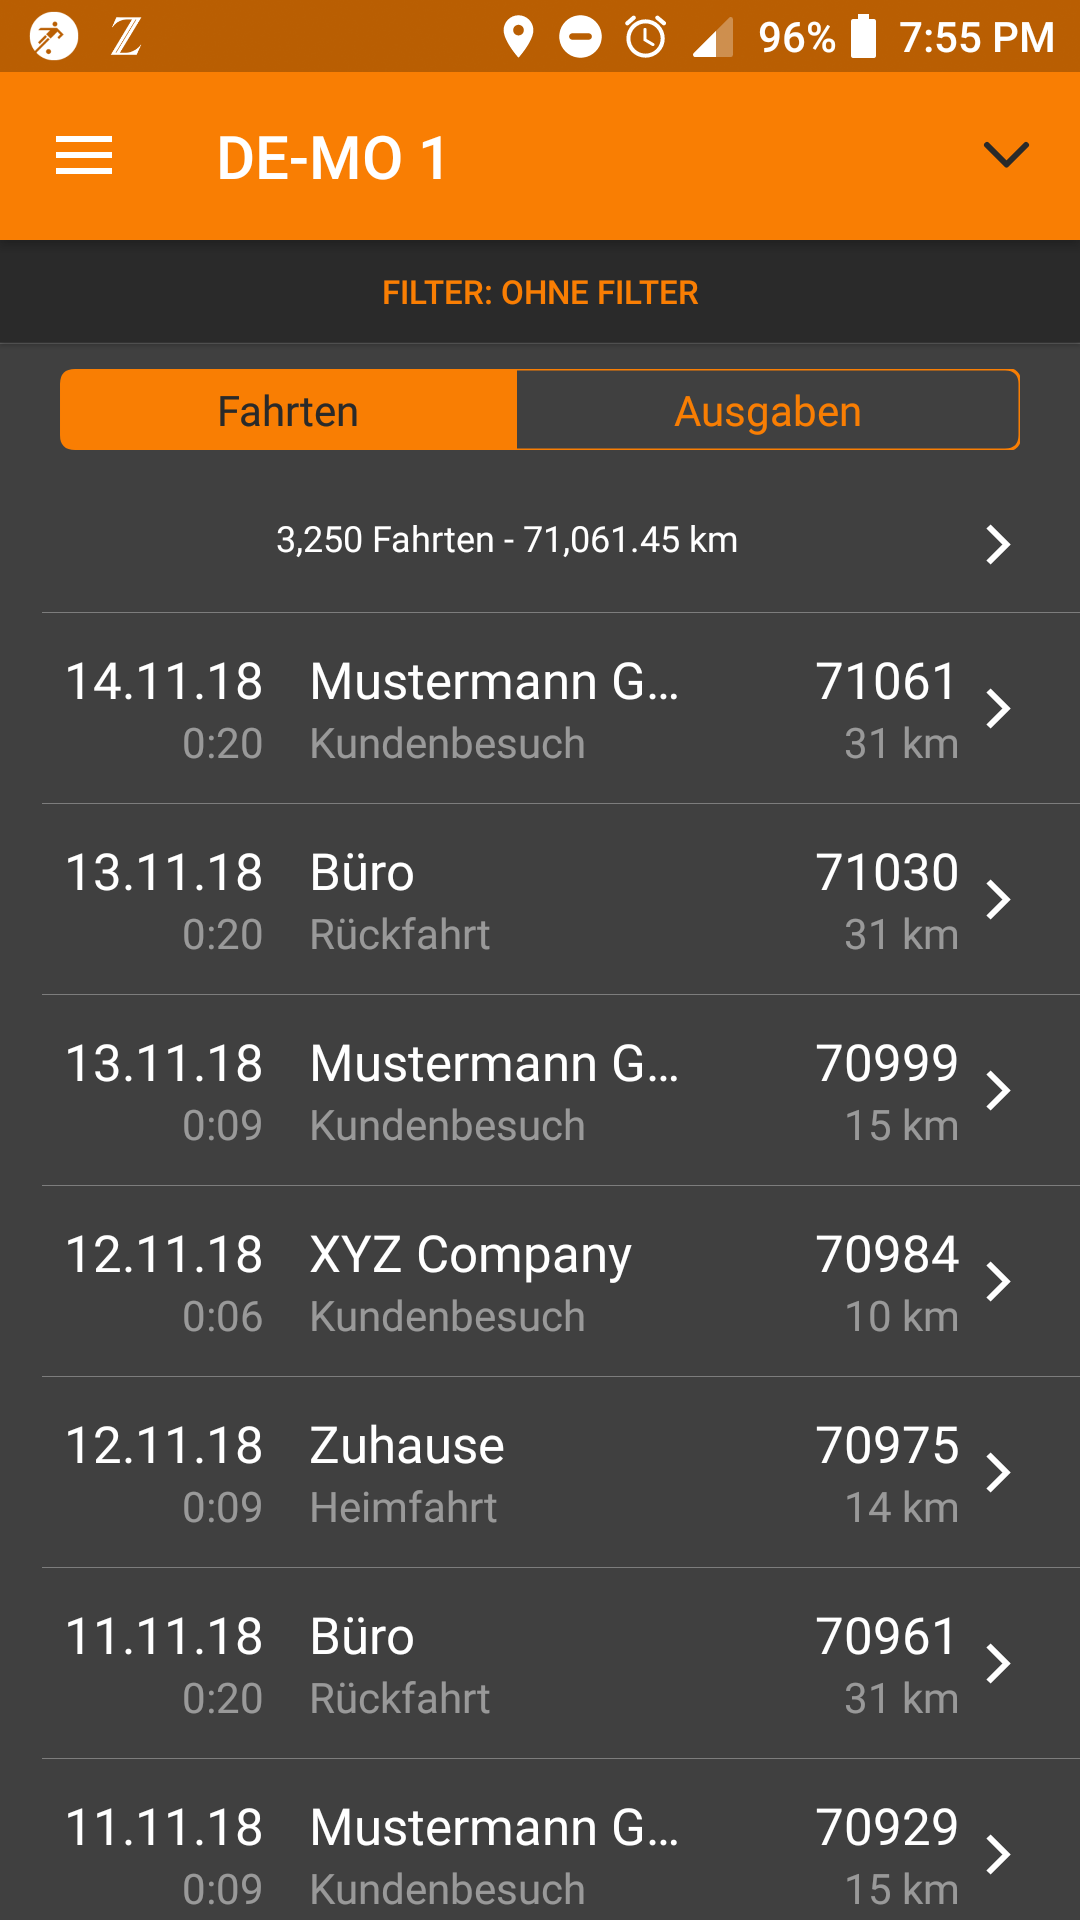
\includegraphics[scale=0.14]{img/pro1}
        \caption{\label{img:img/pro1}Driverslog Pro 2 - Fahrtenbuch, Listenansicht}
    \end{minipage}
    \hspace{0.1\linewidth}% Abstand zwischen Bilder
    \begin{minipage}[b]{.4\linewidth} % [b] => Ausrichtung an \caption
        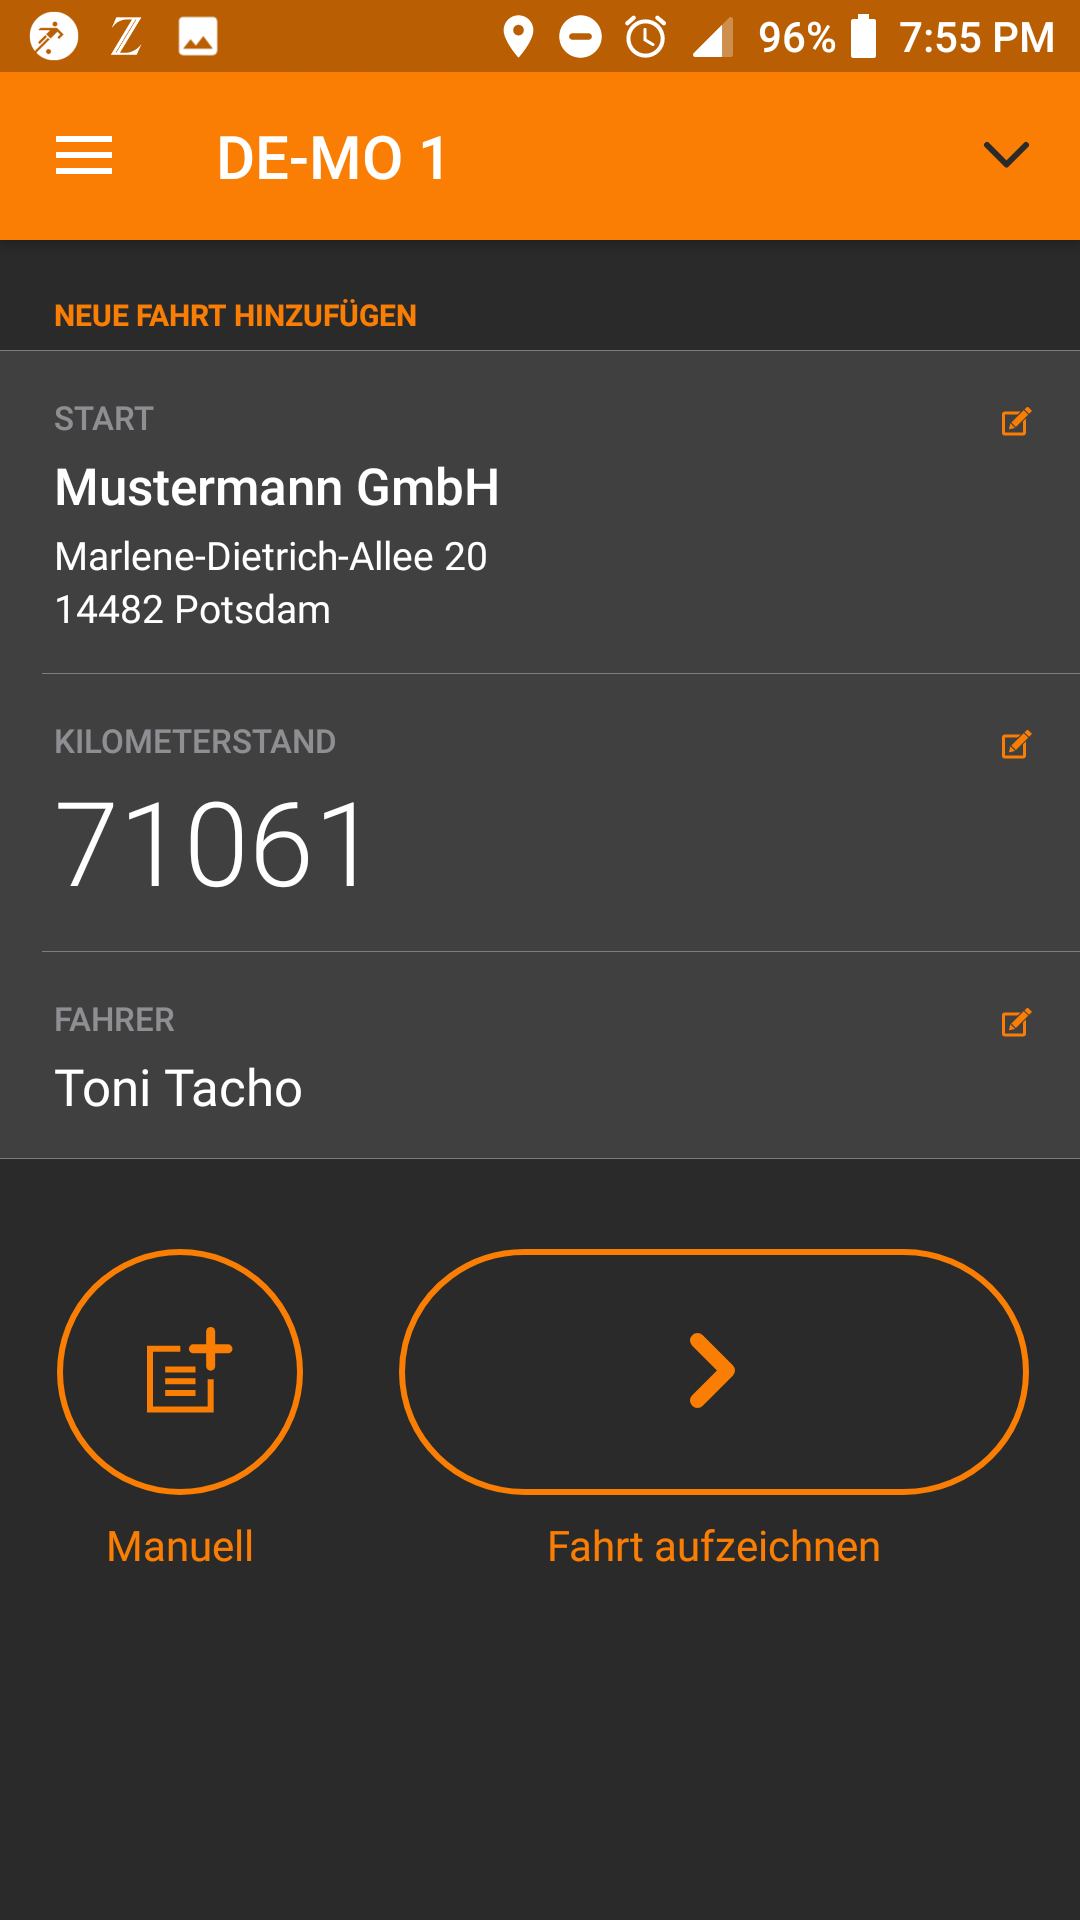
\includegraphics[scale=0.14]{img/pro2}
        \caption{\label{img:img/pro2}Driverslog Pro 2 - Fahrtenbuch, Fahrt hinzufügen}
    \end{minipage}
\end{figure}

\begin{figure}[H]%zwei bilder nebeneinander
    \begin{minipage}[b]{.4\linewidth} % [b] => Ausrichtung an \caption
        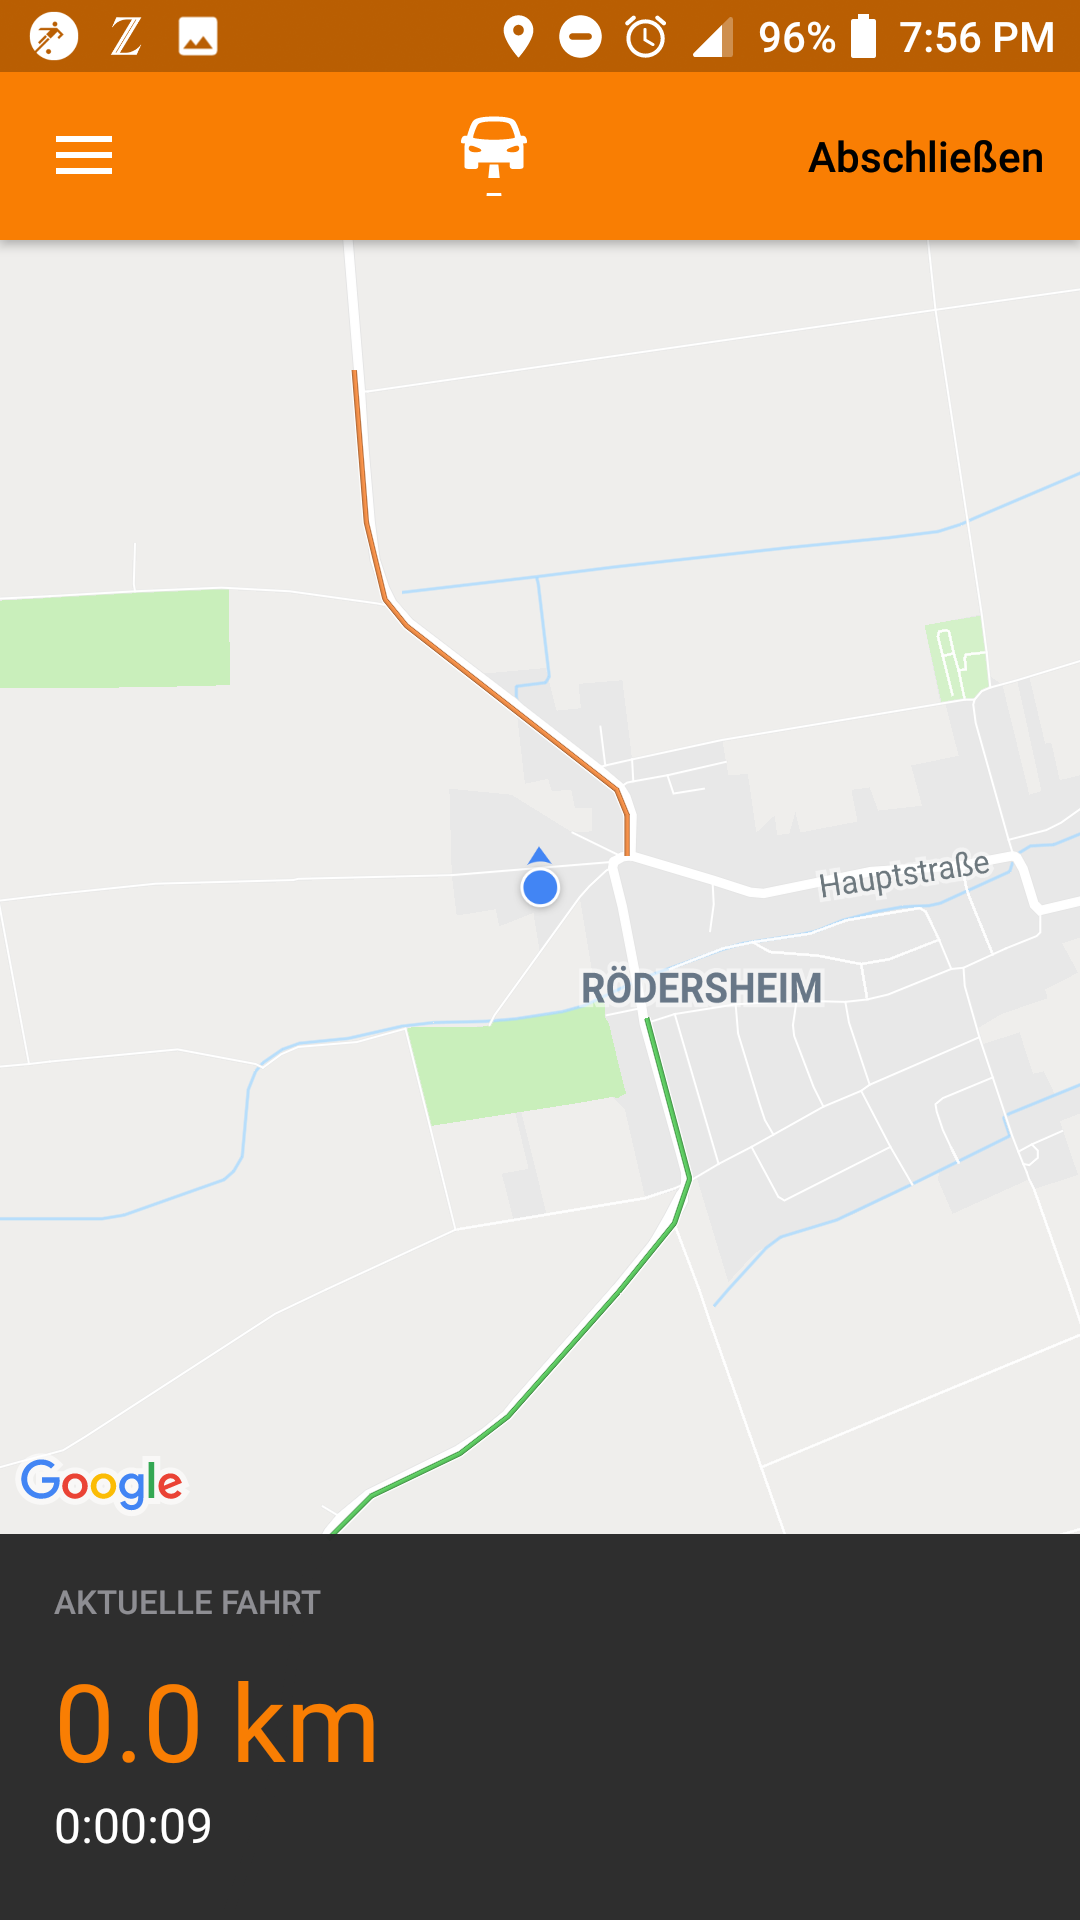
\includegraphics[scale=0.14]{img/pro3}
        \caption{\label{img:img/pro3}Driverslog Pro 2 - Fahrtenbuch, Fahrt aufzeichnen}
    \end{minipage}
    \hspace{0.1\linewidth}% Abstand zwischen Bilder
    \begin{minipage}[b]{.4\linewidth} % [b] => Ausrichtung an \caption
        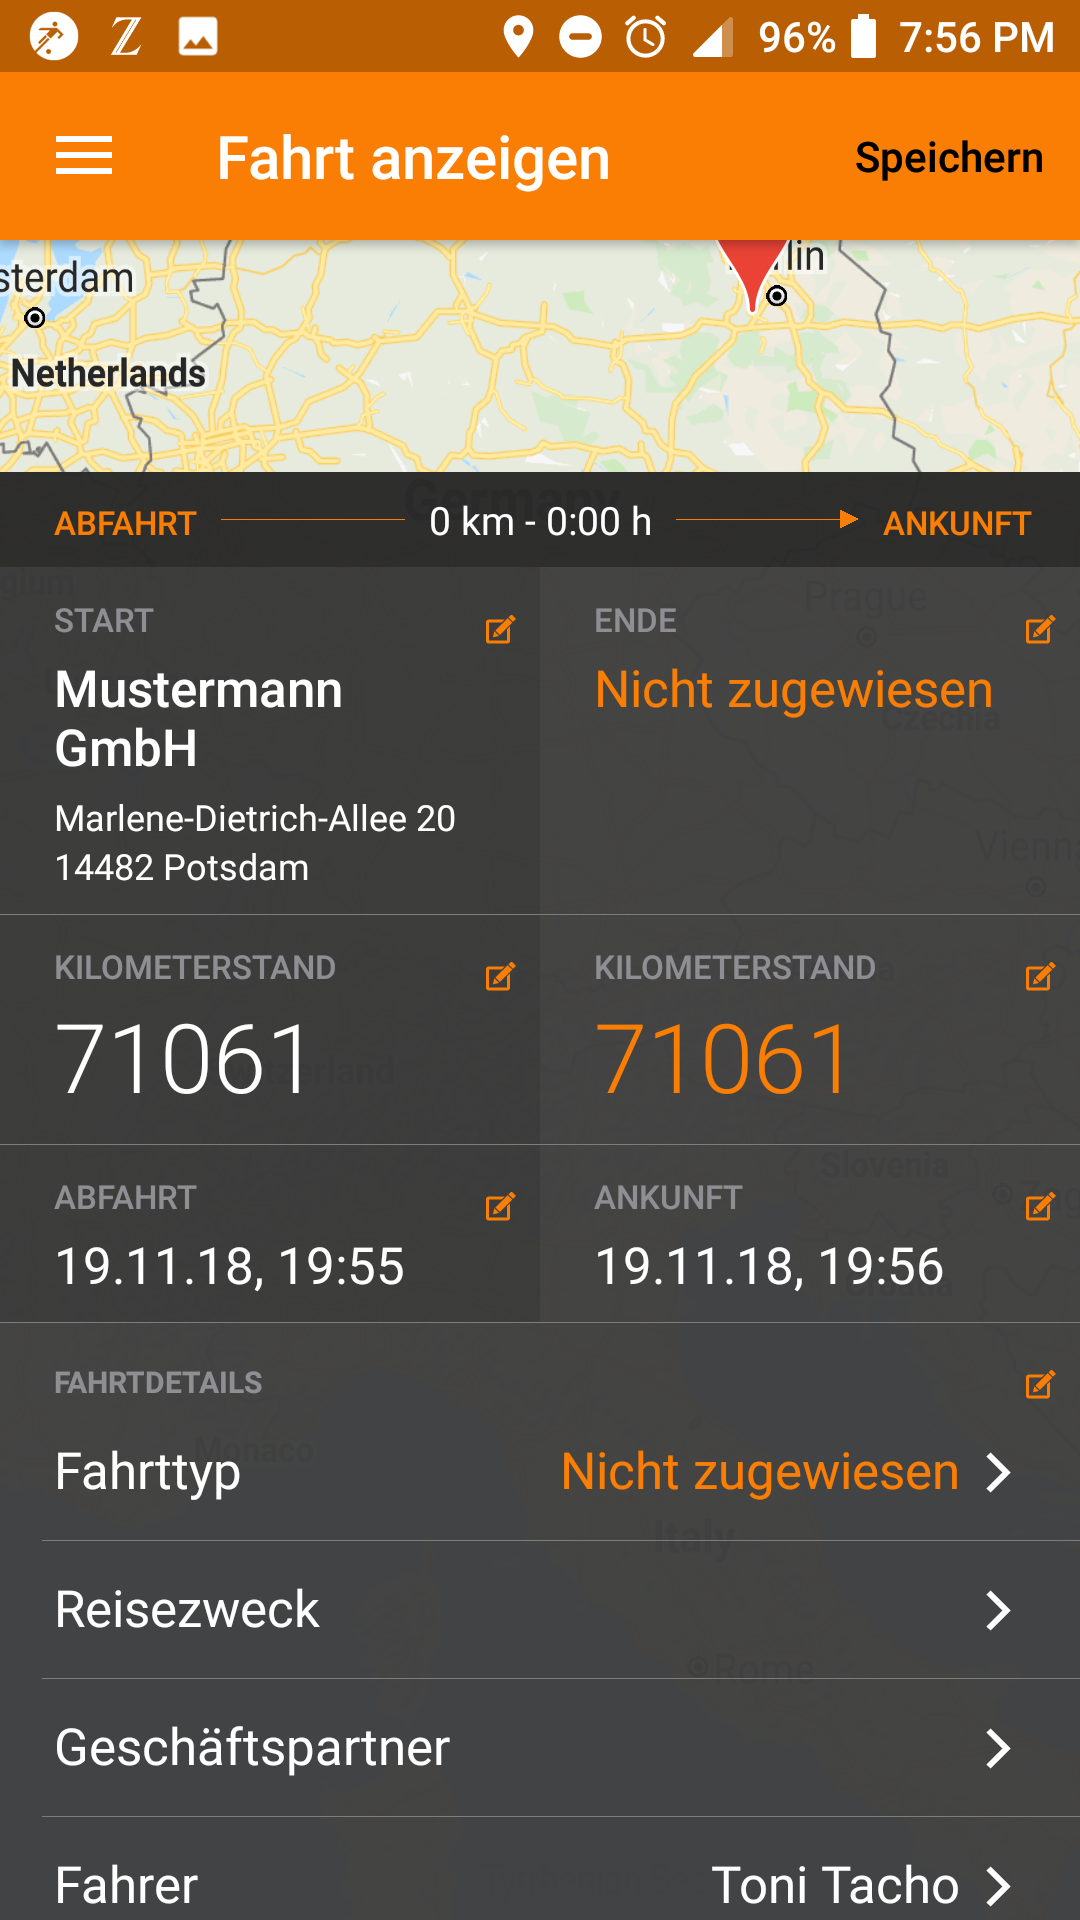
\includegraphics[scale=0.14]{img/pro4}
        \caption{\label{img:img/pro4}Driverslog Pro 2 - Fahrtenbuch, Fahrt anlegen}
    \end{minipage}
\end{figure}


\begin{figure}[H]
        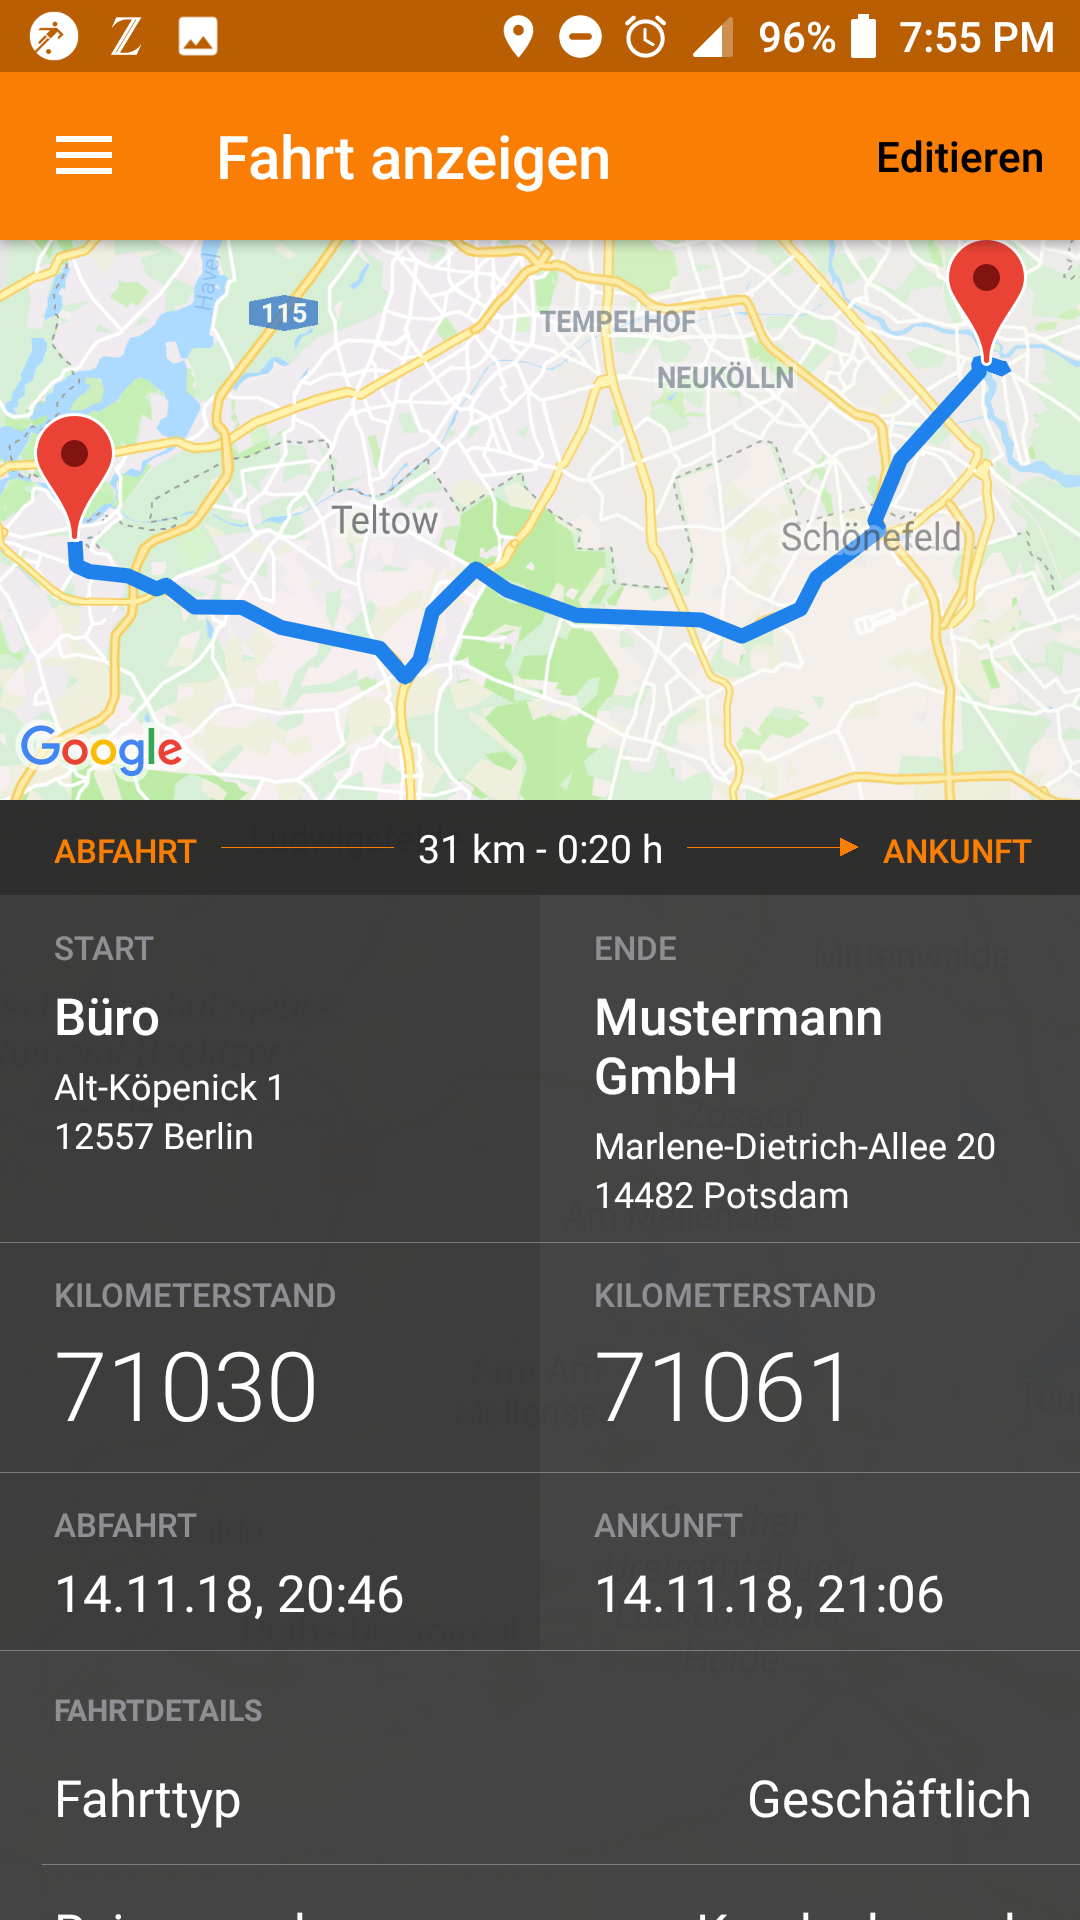
\includegraphics[scale=0.14]{img/pro5}
        \caption{\label{img:img/pro5}Driverslog Pro 2 - Fahrtenbuch, Detailansicht}
\end{figure}


\subsubsection{Kommentare im Play Store}
\begin{enumerate}
    \item
\end{enumerate}

\subsubsection{Fazit}
Diese App benutzt die selbe Oberfläche um Fahrten zu erfassen, hinzuzügen und für die Detailansicht

\subsection{Fazit}
Generell lässt sich sagen das es im Play Store eher wenige Apps gibt.
